% Adapted from catskillsresearch/lyasoff2016 scripts/tex_preamble_arxiv.tex (Lean listings removed).
\documentclass[11pt,a4paper]{article}

\usepackage[utf8]{inputenc}
\usepackage[T1]{fontenc}
\usepackage{lmodern}
\usepackage[margin=1in]{geometry}
\usepackage{amsmath}
\usepackage{amssymb}
\usepackage{bm}
\usepackage{booktabs}
\usepackage{array}
\usepackage{tabularx}
\usepackage{authblk}
\usepackage{xcolor}
\usepackage{graphicx}
\usepackage[export]{adjustbox}
\usepackage{float}
\usepackage{longtable}
\usepackage{calc}
\usepackage{newunicodechar}
\usepackage{xurl}
\usepackage{caption}
\captionsetup{font=small,labelfont=bf}
\usepackage[numbers,sort&compress]{natbib}
\usepackage[colorlinks=true,linkcolor=blue!40!black,citecolor=blue!40!black,urlcolor=blue!40!black]{hyperref}
% The narrative already has a References heading; do not add a second one.
\renewcommand{\bibsection}{}
\emergencystretch=2em
\numberwithin{equation}{section}
\setlength{\parskip}{0.35em}

% pandoc helpers
\providecommand{\tightlist}{\setlength{\itemsep}{0pt}\setlength{\parskip}{0pt}}
\makeatletter
\providecommand{\real}[1]{#1}
\makeatother
\setlength{\LTpre}{0.5\baselineskip}
\setlength{\LTpost}{0.5\baselineskip}

\usepackage{fancyhdr}
\pagestyle{fancy}
\fancyhf{}
\fancyfoot[R]{\thepage}
\fancyhead[L]{\small\itshape MAST poloidal flux imputation}
\renewcommand{\headrulewidth}{0pt}
\fancypagestyle{plain}{%
  \fancyhf{}%
  \fancyfoot[C]{\small\textcopyright\ 2026 Lars Warren Ericson (Catskills Research Company). Apache License 2.0.}%
  \fancyfoot[R]{\thepage}%
  \renewcommand{\headrulewidth}{0pt}%
}

% --- Unicode used in the prose (pdfLaTeX needs every non-ASCII glyph declared) ---
\newunicodechar{α}{\ensuremath{\alpha}}
\newunicodechar{β}{\ensuremath{\beta}}
\newunicodechar{γ}{\ensuremath{\gamma}}
\newunicodechar{δ}{\ensuremath{\delta}}
\newunicodechar{κ}{\ensuremath{\kappa}}
\newunicodechar{λ}{\ensuremath{\lambda}}
\newunicodechar{μ}{\ensuremath{\mu}}
\newunicodechar{ρ}{\ensuremath{\rho}}
\newunicodechar{σ}{\ensuremath{\sigma}}
\newunicodechar{τ}{\ensuremath{\tau}}
\newunicodechar{φ}{\ensuremath{\varphi}}
\newunicodechar{ψ}{\ensuremath{\psi}}
\newunicodechar{Δ}{\ensuremath{\Delta}}
\newunicodechar{Ω}{\ensuremath{\Omega}}
\newunicodechar{ℓ}{\ensuremath{\ell}}
\newunicodechar{≥}{\ensuremath{\geq}}
\newunicodechar{≤}{\ensuremath{\leq}}
\newunicodechar{≈}{\ensuremath{\approx}}
\newunicodechar{≠}{\ensuremath{\neq}}
\newunicodechar{×}{\ensuremath{\times}}
\newunicodechar{−}{\ensuremath{-}}
\newunicodechar{±}{\ensuremath{\pm}}
\newunicodechar{→}{\ensuremath{\rightarrow}}
\newunicodechar{←}{\ensuremath{\leftarrow}}
\newunicodechar{∩}{\ensuremath{\cap}}
\newunicodechar{∪}{\ensuremath{\cup}}
\newunicodechar{∅}{\ensuremath{\emptyset}}
\newunicodechar{⊆}{\ensuremath{\subseteq}}
\newunicodechar{∈}{\ensuremath{\in}}
\newunicodechar{∫}{\ensuremath{\int}}
\newunicodechar{∮}{\ensuremath{\oint}}
\newunicodechar{∇}{\ensuremath{\nabla}}
\newunicodechar{∞}{\ensuremath{\infty}}
\newunicodechar{√}{\ensuremath{\surd}}
\newunicodechar{⟨}{\ensuremath{\langle}}
\newunicodechar{⟩}{\ensuremath{\rangle}}
\newunicodechar{·}{\ensuremath{\cdot}}
\newunicodechar{²}{\textsuperscript{2}}
\newunicodechar{³}{\textsuperscript{3}}
\newunicodechar{✓}{\ensuremath{\checkmark}}
\newunicodechar{…}{\ldots}
\newunicodechar{§}{\S}

\hypersetup{pdftitle={MAST Poloidal Flux Imputation in the Absence of Direct Magnetic Sensors},pdfauthor={Lars Warren Ericson}}


\title{\textbf{MAST Poloidal Flux Imputation in the Absence of Direct Magnetic Sensors}}
\author[1]{\textbf{Lars Warren Ericson}}
\affil[1]{Catskills Research Company}
\affil[1]{\url{https://github.com/catskillsresearch/mast-flux-imputation}}
\affil[1]{\texttt{lars.ericson@catskillsresearch.com}}
\date{\today}

\begin{document}
\maketitle
\begin{center}\small\textbf{ORCID:} 0000-0001-8299-9361\end{center}
\begin{abstract}
We reconstruct the poloidal magnetic flux \(\psi(R,Z)\) of MAST plasmas on a \(65\times65\) grid, together with the edge safety factor \(q_{95}\) and the normalised beta \(\beta_N\), using only the poloidal-field coil currents, the plasma current \(I_p\), the toroidal-field current and midplane Thomson scattering. No magnetic probe or flux-loop signal enters either model. Two models are described. OSF is a free-boundary Grad--Shafranov forward solver: an elliptic-integral Green's-function vacuum field over the 812-element MAST coil set, a prescribed-shape current density fixed by an Ampère constraint and iterated to self-consistency, a flux-surface integral for \(q_{95}\) and a Thomson pressure moment for \(\beta_N\). M9 is a PCA-basis neural surrogate: a residual network maps measured inputs to 60 principal-component coefficients of EFIT++ flux, trained on 3,622 FAIR-MAST archive shots; despite its legacy file name it is not physics-informed. On a sealed, seed-42 holdout of FAIR-MAST shots disjoint from M9 training (65 shots, 3,449 diverted frames), scored with the Fusion Equilibrium Challenge metric, OSF reaches \(S=0.618634\) (\(R^2_\psi=0.917210\)) and the hybrid M9 + OSF reaches \(S=0.862677\) (\(R^2_\psi=0.997771\), \(1-D_{\rm LCFS}=0.945207\)), while \(q_{95}\) and \(\beta_N\) remain weak (\(R^2=0.342298\) and \(0.394260\)). We document exactly what each component was fitted to, including where earlier project documentation disagrees with the code, and propose an automated failure-mode audit to replace visual inspection when training at archive scale.
\end{abstract}
\clearpage
\tableofcontents
\clearpage

\hypertarget{introduction}{%
\clearpage
\section{Introduction}\label{introduction}}

\hypertarget{problem-statement}{%
\subsection{Problem statement}\label{problem-statement}}

Equilibrium reconstruction recovers the axisymmetric magnetic equilibrium of a tokamak plasma from measurements. The standard tool, EFIT \cite{lao1985} and its MAST implementation EFIT++ \cite{appel2006}, fits the Grad--Shafranov equation \cite{shafranov1958,grad1958} to magnetic probes and flux loops, optionally constrained by kinetic and internal-field data. The magnetic sensors carry most of the information about the plasma boundary.

The Fusion Equilibrium Challenge (FEC) \cite{fec2026dataset,fec2026starter} poses the inverse question: how much of \(\psi(R,Z)\) can be recovered \emph{without} direct magnetic sensors? Its MAST \cite{darke1995,sykes2001,lloyd2003} inputs are the actuator currents (solenoid, P2--P6 upper/lower poloidal-field circuits, the toroidal-field coil and the EFPS circuit), the plasma current \(I_p\), and the core and edge Thomson scattering profiles \(T_e(R), n_e(R)\) on the horizontal midplane \cite{scannell2010}. The targets are the EFIT++ flux map on a fixed \(65\times65\) \((R,Z)\) grid, \(q_{95}\) and \(\beta_N\) at each EFIT time.

This paper describes, at the level of the code, a MAST-only system for this task extracted into the repository \nolinkurl{catskillsresearch/mast-flux-imputation}, and reports its measured performance on a sealed archive holdout.

\hypertarget{contributions}{%
\subsection{Contributions}\label{contributions}}

\begin{enumerate}
\def\labelenumi{\arabic{enumi}.}
\item
  A complete mathematical description of OSF (\nolinkurl{mast_12_osf_0.0.12}), a free-boundary Grad--Shafranov forward solver driven by measured currents, separating machine constants from the 38 calibrated parameters (Section 3).
\item
  An exact description of M9 (\texttt{M9\_win50}), an ensemble of three PCA-basis neural surrogates of EFIT++ flux trained on FAIR-MAST \cite{jackson2024fairmast}, and an explicit statement that it is \emph{not} a physics-informed neural network: its loss has no Grad--Shafranov residual (Section 4).
\item
  A reproducible build: data acquisition, ingest, quality control, holdout construction with a disjointness proof, training, prediction, scoring and a browser viewer (Section 5).
\item
  Measured results on a sealed 80-shot holdout, re-derived from the saved prediction files and cross-checked against an independent implementation of the scorer (Section 7).
\item
  An honest provenance audit, listing where earlier documentation and the code disagree, and a proposal for an automated failure-mode audit to sharpen training (Sections 8--9).
\end{enumerate}

\hypertarget{related-work}{%
\subsection{Related work}\label{related-work}}

Free-boundary equilibrium solvers based on Green's functions of the Grad--Shafranov operator and Picard iteration go back to \cite{lackner1976}; textbook treatments are given by \cite{freidberg1987,freidberg2014,jardin2010,wesson2011}. Neural networks have been used as Grad--Shafranov solvers \cite{vanmilligen1995} and, constrained by measured magnetic signals, for fast reconstruction \cite{joung2020}. Physics-informed neural networks (PINNs) \cite{raissi2019} add a PDE residual to the training loss; the M9 model below does not. Reduced-order representations of fields by principal component analysis / proper orthogonal decomposition \cite{pearson1901,hotelling1933,berkooz1993} underlie the M9 output space.

\hypertarget{data}{%
\clearpage
\section{Data}\label{data}}

Two public sources are used: the FEC MAST split and the FAIR-MAST archive from which the challenge itself was built. Both carry EFIT++ reconstructions as labels; the models only ever see inputs.

\hypertarget{fusion-equilibrium-challenge-mast-data}{%
\subsection{Fusion Equilibrium Challenge MAST data}\label{fusion-equilibrium-challenge-mast-data}}

The FEC dataset \cite{fec2026dataset} (CC BY 4.0) stores one Parquet row per shot with nested arrays for every time series. Its MAST portion used here consists of

\begin{itemize}
\item
  \texttt{mast\_public\_test}: 1,206 shots with inputs only (labels withheld for the leaderboard);
\item
  three labelled starter-kit shots, 28348, 28350 and 28351 (36, 42 and 37 EFIT frames), distributed with the starter kit \cite{fec2026starter} and fetched with \texttt{data/fec/fetch.py\ -\/-demo} (sha256-pinned).
\end{itemize}

FEC keeps only \emph{diverted} EFIT time slices. For MAST a slice is diverted when EFIT++ reports an X-point (\texttt{efm/xpoint\{1,2\}}); the challenge reports that this keeps 66.4\% of MAST frames \cite{fec2026dataset}. The input time series are not subset, so \texttt{efit\_times} is not contiguous.

\hypertarget{fair-mast-archive-and-ingest}{%
\subsection{FAIR-MAST archive and ingest}\label{fair-mast-archive-and-ingest}}

FAIR-MAST \cite{jackson2024fairmast} publishes the MAST archive as Zarr stores at \nolinkurl{s3://mast/level1/shots/N.zarr} for shot number N (endpoint \nolinkurl{s3.echo.stfc.ac.uk}, anonymous, CC BY-SA 4.0). The ingest (\nolinkurl{data/fair_mast/ingest.py}) reads four groups per shot,

\begin{longtable}[]{@{}lll@{}}
\toprule\noalign{}
group & content & use \\
\midrule\noalign{}
\endhead
\bottomrule\noalign{}
\endlastfoot
\texttt{efm} & EFIT++: \texttt{psirz}, \texttt{q\_95}, \texttt{betan}, X-points & labels only \\
\texttt{amc} & coil and plasma currents & inputs \\
\texttt{ayc} & core Thomson \(T_e, n_e\) & inputs \\
\texttt{aye} & edge Thomson \(T_e, n_e\) & inputs \\
\end{longtable}

and writes one row in the FEC schema plus \texttt{efit\_psirz}. Static tables (coil geometry, chord positions) are copied from a released FEC row; they are given inputs, not labels. 3,738 shots were ingested. For the same shot and time, FAIR-MAST and FEC flux maps are bit-identical; the populations differ only because the archive keeps all slices (ramp-up, limited, ramp-down).

\nolinkurl{data/fair_mast/fetch_efit_labels.py} adds the scalar labels and the diverted flag. Its rule (any finite \texttt{efm/xpoint\{1,2\}\_rc}) reproduces the FEC frame selection on all three demo shots, and its \texttt{q\_95}, \texttt{betan} and edge-Thomson arrays match the FEC demo rows exactly (\nolinkurl{tests/test_labels.py}).

\hypertarget{input-vector-and-clocks}{%
\subsection{Input vector and clocks}\label{input-vector-and-clocks}}

Per shot the model inputs are:

\begin{itemize}
\item
  \textbf{Actuators:} 13 current channels on a 0.2 ms (5 kHz) clock spanning \(-2000\) to \(4000\) ms (30,000 samples): \texttt{sol}, \texttt{p2u}, \texttt{p2l}, \texttt{p3u}, \texttt{p3l}, \texttt{p4u}, \texttt{p4l}, \texttt{p5u}, \texttt{p5l}, \texttt{p6u}, \texttt{p6l}, \texttt{tf}, \texttt{efps} (kA, or kA·turn for the P circuits), plus \(I_p\).
\item
  \textbf{Kinetic profiles:} core Thomson \(T_e, n_e\) on 131 channels at about 2 ms cadence (130 chord radii in the FEC rows) and edge Thomson on 16 channels at \(R\approx1.33\)--\(1.49\) m. All chords lie on the midplane \(Z=0\) \cite{scannell2010}.
\item
  \textbf{Geometry:} the 812-row coil table (656 solenoid rows, 156 P2--P6 elements; centre, width, height), the 146-chord Thomson table and the \(65\times65\) grid \(R\in[0.06,2.00]\) m, \(Z\in[-2,2]\) m.
\item
  \textbf{Output clock:} \texttt{efit\_times} (ms). Inputs are interpolated onto it.
\end{itemize}

There are no magnetic-probe (\(B_\theta\) pick-up) or flux-loop channels. The labels, however, are EFIT++ reconstructions that \emph{were} constrained by those sensors.

\hypertarget{sealed-holdout-and-disjointness}{%
\subsection{Sealed holdout and disjointness}\label{sealed-holdout-and-disjointness}}

The holdout is the split built into the M9 training code. Let \(\mathcal K\) be the sorted list of 3,738 ingested keys and \(\mathcal D\) the three demo shots. Then

\[
\mathcal S = \mathrm{first}_{80}\big(\mathrm{shuffle}_{42}(\mathcal K\setminus\mathcal D)\big),\qquad
\mathcal P = (\mathcal K\setminus\mathcal D)\setminus\mathcal S,\quad |\mathcal P| = 3655,
\]

with \texttt{random.Random(42).shuffle}. Quality control on \(\mathcal P\) keeps 3,622 shots (\(\mathcal Q\)) and quarantines 33. \nolinkurl{data/fair_mast/make_holdout.py} recomputes the split and checks

\begin{longtable}[]{@{}
  >{\raggedright\arraybackslash}p{(\columnwidth - 2\tabcolsep) * \real{0.5000}}
  >{\raggedright\arraybackslash}p{(\columnwidth - 2\tabcolsep) * \real{0.5000}}@{}}
\toprule\noalign{}
\begin{minipage}[b]{\linewidth}\raggedright
check
\end{minipage} & \begin{minipage}[b]{\linewidth}\raggedright
result
\end{minipage} \\
\midrule\noalign{}
\endhead
\bottomrule\noalign{}
\endlastfoot
recomputed \(\mathcal P\) equals the QC training set (keep ∪ quarantine) & true (3,655) \\
QC keep list equals the shipped \nolinkurl{mast_qc_keep.txt} & true (3,622) \\
\(\mathcal Q\cap\mathcal S\), \(\mathcal P\cap\mathcal S\), \(\mathcal D\cap\mathcal S\) & ∅, ∅, ∅ \\
quarantined sealed shot & 27373 ∈ \(\mathcal S\) \\
\end{longtable}

and every M9 checkpoint records \texttt{seed\ =\ 42}, \texttt{train\_shots\ =\ 3622}. The holdout is therefore disjoint from all M9 training and validation data.

\textbf{FEC-protocol cut.} Each sealed shot is restricted to its diverted EFIT slices with the FEC rule; inputs keep their full clocks. Fifteen sealed shots have no diverted slice (24901, 26506, 29932, 24876, 28295, 27681, 23248, 27621, 27720, 29297, 26273, 27819, 27778, 23424, 30442) and are excluded, leaving \textbf{65 shots and 3,449 frames} out of 5,280 EFIT slices. Edge Thomson missing from the ingest is overlaid from \texttt{aye} (60 of 65 shots).

\textbf{Caveat.} OSF was not fitted to these shots' labels, but its global scalar factors were tuned against aggregate leaderboard scores on the public-test fold, and the FAIR-MAST pool likely overlaps the FEC hidden folds (Section 8).

\hypertarget{forward-gradshafranov-model-osf}{%
\clearpage
\section{Forward Grad--Shafranov model (OSF)}\label{forward-gradshafranov-model-osf}}

OSF (\nolinkurl{models/osf}, model id \nolinkurl{mast_12_osf_0.0.12}) computes, independently at every EFIT time, a free-boundary equilibrium driven by the measured currents. It uses no flux label at inference and no fit to measured flux. The block diagram is shown below; the following notes derive each block.

\begin{figure}[H]
\hypertarget{fig:osf}{%
\centering
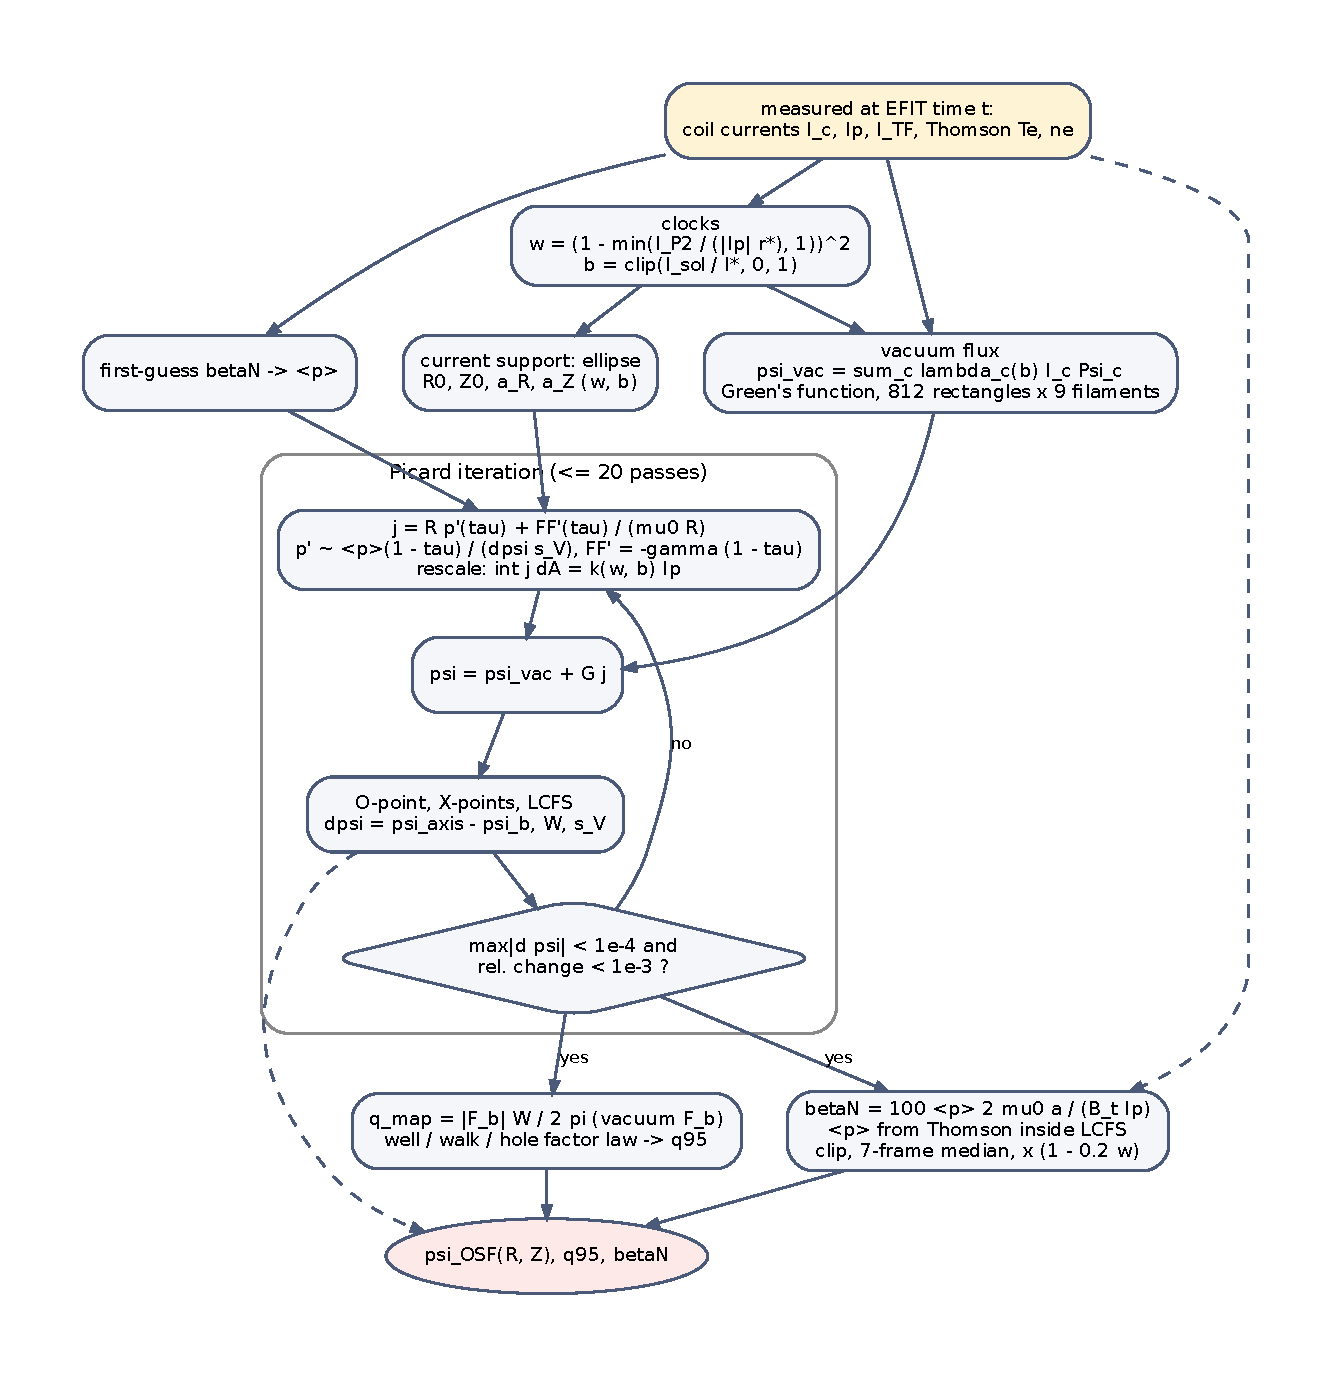
\includegraphics[max width=0.95\linewidth,max height=0.62\textheight,keepaspectratio]{figures/diag_osf_solver.pdf}
\caption{OSF forward-solver block diagram. Everything above the Picard loop is computed once per frame from measured currents; the loop updates the plasma current density until the flux and three scalar diagnostics stop changing.}\label{fig:osf}
}
\end{figure}

\hypertarget{gradshafranov-equation-and-sign-convention}{%
\subsection{Grad--Shafranov equation and sign convention}\label{gradshafranov-equation-and-sign-convention}}

In cylindrical coordinates \((R,\varphi,Z)\) an axisymmetric field is \(\mathbf B = \nabla\psi\times\nabla\varphi + F(\psi)\nabla\varphi\), with \(\psi\) the poloidal flux per radian (Wb rad\(^{-1}\), the FEC convention) and \(F=RB_\varphi\). Force balance \(\mathbf j\times\mathbf B=\nabla p\) with \(p=p(\psi)\) gives the Grad--Shafranov equation \cite{shafranov1958,grad1958,freidberg2014}

\begin{equation}
\Delta^{*}\psi \equiv R\frac{\partial}{\partial R}\Big(\frac{1}{R}\frac{\partial\psi}{\partial R}\Big)+\frac{\partial^{2}\psi}{\partial Z^{2}}
= -\mu_0 R\,j_\varphi = -\mu_0R^2p'(\psi) - F F'(\psi).
\label{eq:gs}
\end{equation}

The toroidal current density is therefore \(j_\varphi = R\,p'(\psi) + FF'(\psi)/(\mu_0R)\).

\textbf{Sign convention.} In the EFIT++/FAIR-MAST data the magnetic axis is a \emph{maximum} of \(\psi\); we write \(\sigma_{\rm ax}=+1\) (DIII-D in the same challenge uses \(-1\)). OSF solves directly in this convention (\texttt{sigma\_ax\ =\ 1}), so its output needs no sign flip, and the scorer's global sign probe selects \(s=+1\) on every run reported here.

\textbf{Free-boundary form.} With the Green's function \(G\) of \(\Delta^*\) (next note) the solution in the whole domain is

\begin{equation}
\psi(\mathbf x) = \psi_{\rm vac}(\mathbf x) + \int_{\Omega_p} G(\mathbf x,\mathbf x')\,j_\varphi(\mathbf x')\,dA',
\label{eq:freeb}
\end{equation}

where \(\psi_{\rm vac}\) is generated by the external coils and \(\Omega_p\) is the support of the plasma current \cite{lackner1976,jardin2010}. Vessel and passive-structure eddy currents are not modelled.

\hypertarget{vacuum-flux-from-the-coil-set}{%
\subsection{Vacuum flux from the coil set}\label{vacuum-flux-from-the-coil-set}}

The flux per radian at \((R,Z)\) from a coaxial circular filament of radius \(R'\) at height \(Z'\) carrying current \(I\) is \cite{jacksonCED1999,lackner1976}

\begin{equation}
\psi = I\,G(R,Z;R',Z'),\qquad
G = \frac{\mu_0\sqrt{RR'}}{2\pi k}\Big[(2-k^{2})K(k)-2E(k)\Big],\qquad
k^{2}=\frac{4RR'}{(R+R')^{2}+(Z-Z')^{2}},
\label{eq:green}
\end{equation}

with \(K\) and \(E\) the complete elliptic integrals of the first and second kind \cite{abramowitz1964} (SciPy \texttt{ellipk}, \texttt{ellipe} with parameter \(m=k^2\)). \(G\) is set to 0 on the axis \(R=0\) and \(k^2\) is clipped below 1 to avoid the logarithmic singularity at coincident points.

The FEC MAST coil table has 812 rectangular elements: 656 solenoid rows, each one turn carrying \(I_{\rm sol}\), and 156 elements of the P2--P6 upper/lower circuits, each carrying its circuit's ampere-turns divided by the number of elements of that circuit. Each rectangle of width \(w\) and height \(h\) is replaced by the mean of \(3\times3\) filaments at offsets \(\{-1,0,1\}\cdot w/3\), \(\{-1,0,1\}\cdot h/3\). This gives one unit map \(\Psi_c(R,Z)\) per circuit \(c\), and

\begin{equation}
\psi_{\rm vac}(R,Z) = \sum_{c}\lambda_c(b)\,I_c\,\Psi_c(R,Z).
\label{eq:vac}
\end{equation}

The TF and EFPS circuits do not enter \(\psi_{\rm vac}\). The multipliers \(\lambda_c\) are calibrated functions of the bleed clock \(b\) (next note):

\begin{longtable}[]{@{}ll@{}}
\toprule\noalign{}
circuit & multiplier \\
\midrule\noalign{}
\endhead
\bottomrule\noalign{}
\endlastfoot
P2 upper and lower & \(\lambda_V = 1.8 - b\) \\
P2 lower, additionally & \(\times\,(1+0.105(1-b))\) \\
P4 pair & \(1.15\) \\
P5 pair & \(\times\,(1-0.18(1-b))\) \\
solenoid & \(0.5+0.10\,b\) \\
P3, P6 & 1 \\
\end{longtable}

The plasma term in \eqref{eq:freeb} uses the same kernel evaluated between grid nodes, assembled once as a \(4225\times4225\) matrix including the cell area \(\Delta R\,\Delta Z\).

\hypertarget{walk-and-bleed-clocks}{%
\subsection{Walk and bleed clocks}\label{walk-and-bleed-clocks}}

A MAST discharge moves from a solenoid-driven start-up towards a diverted flat-top. OSF summarises the phase with two dimensionless ``clocks'' computed from the measured currents at each EFIT time:

\begin{equation}
w = \Big(1-\min\Big(\frac{\bar I_{P2}}{|I_p|\,r_\star},\,1\Big)\Big)^{2},\qquad
\bar I_{P2}=\tfrac12\big(|I_{P2U}|+|I_{P2L}|\big),\qquad
b = \mathrm{clip}\Big(\frac{I_{\rm sol}}{I_\star},0,1\Big),
\label{eq:clocks}
\end{equation}

with \(r_\star=0.34\) and \(I_\star=16.3\) kA. The divertor ``walk'' \(w\) approaches 1 as the P2 current becomes small relative to \(I_p\); the solenoid ``bleed'' \(b\) is 1 while the solenoid still carries positive current and 0 once it has swung through zero. In the code these clocks set the current support, the coil multipliers, the enclosed-current factor and the read-out laws. They are not fitted per shot; they are deterministic functions of the actuators, which is how OSF blends limited-like and diverted-like behaviour without a classifier.

\hypertarget{current-density-ansatz-and-ampuxe8re-constraint}{%
\subsection{Current-density ansatz and Ampère constraint}\label{current-density-ansatz-and-ampuxe8re-constraint}}

\textbf{Support.} The plasma current is confined to a fixed ellipse \(\Omega_p\) (the alternative D-shaped support of the source code is disabled for MAST, \texttt{USE\_VACUUM\_XD\ =\ False}):

\[
\begin{aligned}
R_0 &= 0.82+0.10\,w-0.02\,b, & Z_0 &= 0.009-0.004\,b,\\
a_R &= 0.50+0.08\,w, & a_Z &= a_R+0.08+0.42\,b+0.18\,(1-b),
\end{aligned}
\]

all in metres, with the geometric normalised radius \(\tau=\rho^2=((R-R_0)/a_R)^2+((Z-Z_0)/a_Z)^2\in[0,1]\) on \(\Omega_p\). \(\tau\) is geometric, not a function of \(\psi\): the current shape is held fixed so that it cannot chase an outboard maximum.

\textbf{Profiles.} With \(s_V\) the volume average over \(\Omega_p\) of \(s(\tau)=\tfrac12(1-\tau)^2\) (the integral of the pressure-derivative shape from \(\tau\) to 1) and \(\Delta\psi=\psi_{\rm ax}-\psi_b\),

\begin{equation}
p'(\tau) = \frac{\langle p\rangle\,(1-\tau)}{\Delta\psi\,s_V},\qquad
FF'(\tau) = -\bar\gamma\,(1-\tau),\quad \bar\gamma=-1,\qquad
j_\varphi = R\,p' + \frac{FF'}{\mu_0R}\ \text{ on }\Omega_p .
\label{eq:jphi}
\end{equation}

The pressure scale comes from a first-guess normalised beta \(\beta_N^{(0)}\),

\[
\langle p\rangle = \frac{\beta_N^{(0)}}{100}\,\frac{B_t}{2\mu_0}\,\frac{I_p[\mathrm{MA}]}{a_R},
\]

where \(\beta_N^{(0)}\) is computed from the median Thomson pressure \(2n_eT_e e\) over chords with \(R\in[0.25,1.45]\) m, clipped to \([0.2,4]\) (default 1.3 when no chord is valid).

\textbf{Ampère constraint.} The amplitude is then rescaled so that the enclosed current matches a calibrated fraction of the measured plasma current:

\begin{equation}
\int_{\Omega_p} j_\varphi\,dA = k\,I_p,\qquad k = 0.70+0.30\,w+0.15\,b+0.20\,(1-b).
\label{eq:ampere}
\end{equation}

The factor \(k\ne1\) absorbs, in an averaged way, the current that a fixed ellipse misplaces and the missing vessel currents. Only the \emph{ratio} of the \(p'\) and \(FF'\) terms survives the rescaling, so the pressure guess shapes the current but does not set its total.

\hypertarget{picard-iteration}{%
\subsection{Picard iteration}\label{picard-iteration}}

Because \(p'\) in \eqref{eq:jphi} depends on \(\Delta\psi\) and \(s_V\), and the read-outs depend on the flux-surface geometry, the solve is a fixed-point (Picard) iteration. Starting from \(\psi^{(0)}=\psi_{\rm vac}\), pass \(n\):

\begin{enumerate}
\def\labelenumi{\arabic{enumi}.}
\item
  locate the O-point and the last closed surface of \(\psi^{(n-1)}\); if they are acceptable, set \(\Delta\psi\) from them and \(W=\oint d\ell/(R|\nabla\psi|)\) on the 95\% surface, otherwise fall back to the maximum of \(\psi\) inside \(\Omega_p\) and the mean outside;
\item
  evaluate \(j_\varphi\) from \eqref{eq:jphi} and rescale it with \eqref{eq:ampere};
\item
  update \(\psi^{(n)} = \psi_{\rm vac} + G\,j_\varphi\).
\end{enumerate}

The loop stops when \(\max|\psi^{(n)}-\psi^{(n-1)}|<10^{-4}\) Wb rad\(^{-1}\) \emph{and} the relative changes of \(W\), \(\Delta\psi\) and \(s_V\) are all below \(10^{-3}\), or after 20 passes. Earlier project documents called OSF ``one-shot''; that is accurate only in the sense that nothing is fitted to measured flux --- numerically it is an iteration of up to 20 linear solves per frame.

\hypertarget{magnetic-topology-o-point-x-points-lcfs}{%
\subsection{Magnetic topology: O-point, X-points, LCFS}\label{magnetic-topology-o-point-x-points-lcfs}}

The magnetic axis is the maximum of \(\psi\) (since \(\sigma_{\rm ax}=+1\)) inside the box \(R\in[0.65,1.05]\) m, \(|Z|\le0.5\) m. During the iteration the last closed surface is the outermost compact closed contour around the axis (elongation \(\le2.6\), vertical span \(\le2.8\) m, outer radius \(\ge1.0\) m, inner radius \(\le0.4\) m); candidate X-points are saddles in \(R\in[0.25,1.5]\) m with \(|Z|\ge0.4\) m.

For the read-outs, OSF calls the \emph{scorer's} LCFS extractor (\nolinkurl{fec_scoring/lcfs.py}, marching squares via scikit-image \cite{vanderwalt2014}) restricted by the MAST vessel envelope \nolinkurl{mast_envelope.npz} (\texttt{mask\_coarse}). Earlier documentation stated that the envelope mask was not used; it is used here, in the \(q_{95}\) and \(\beta_N\) read-outs only. If the scorer extractor fails, OSF falls back to its own closed-contour search.

\hypertarget{safety-factor-read-out}{%
\subsection{Safety factor read-out}\label{safety-factor-read-out}}

For a flux surface the safety factor is \(q = \frac{F}{2\pi}\oint\frac{d\ell}{R^{2}B_p} = \frac{F}{2\pi}\oint\frac{d\ell}{R\,|\nabla\psi|}\) \cite{freidberg2014,wesson2011}. OSF evaluates the geometric integral on the 95\% surface \(\psi=\psi_{\rm ax}-0.95\,\Delta\psi\),

\begin{equation}
W=\oint_{\psi_{95}}\frac{d\ell}{R\,|\nabla\psi|},\qquad q_{\rm map} = \frac{|F_b|\,W}{2\pi},\qquad
F_b = \frac{\mu_0N_{\rm TF}I_{\rm TF}}{2\pi},\ N_{\rm TF}=24,
\label{eq:qmap}
\end{equation}

with \(F_b\) the \emph{vacuum} toroidal function (no plasma dia/paramagnetism). Because \(\psi\) is not fully self-consistent, \(q_{\rm map}\) is corrected by a calibrated factor law in the clocks:

\begin{equation}
\begin{aligned}
u&=\mathrm{clip}\Big(\frac{q_{\rm map}-8}{17-8},0,1\Big),\qquad
d = 1+0.35\,(1-w)(1-b),\qquad
h = 2\,b(1-b)^{3},\\
q_{95} &= \big(0.55\,u + (1-u)\,d + h\big)\,q_{\rm map}.
\end{aligned}
\label{eq:qlaw}
\end{equation}

The ``well'' weight \(u\) is 1 while the surface is long (ohmic phase), \(d\) raises \(q\) in the diverted phase, and \(h\) is a bump at the solenoid swing. If no closed surface is found the cylindrical estimate \(q^{*} = 5a^{2}|B_t|/(R_0 I_p[\mathrm{MA}])\) is returned. Earlier documents describe a ``paramagnetic \(c=1.20\) baseline''; no such term exists in the solver. The hybrid mode multiplies the OSF value by \(c^{*}/1.20\) (Section 5).

\hypertarget{normalised-beta-read-out}{%
\subsection{Normalised beta read-out}\label{normalised-beta-read-out}}

The Troyon-normalised beta \cite{troyon1984} is \(\beta_N = 100\,\beta_t\,a\,B_t/I_p[\mathrm{MA}]\) with \(\beta_t = 2\mu_0\langle p\rangle/B_t^{2}\), i.e.

\begin{equation}
\beta_N = \frac{100\,\langle p\rangle\,2\mu_0\,a}{B_t\,I_p[\mathrm{MA}]},\qquad B_t = F_b/R_0 .
\label{eq:betan}
\end{equation}

OSF estimates \(\langle p\rangle\) as the mean of \(2n_eT_e e\) (equal ion and electron pressure assumed) over Thomson chords, interpolated to the EFIT time, whose radius lies inside the extracted LCFS, \(R\in[r_{\rm in},r_{\rm out}]\), with \(a=(r_{\rm out}-r_{\rm in})/2\). Per frame the value is clipped to \([0.2,4]\); over the shot a 7-frame running median removes single laser spikes, and the result is multiplied by \((1-0.2\,w)\). The pressure is a midplane line average, not a volume average, which is one reason the \(\beta_N\) skill is limited (Section 7).

\hypertarget{machine-constants-versus-calibrated-parameters}{%
\subsection{Machine constants versus calibrated parameters}\label{machine-constants-versus-calibrated-parameters}}

\nolinkurl{models/osf/calibration.py} splits the symbols of the source file into four groups. The values are copied exactly; there is no fitting code.

\begin{longtable}[]{@{}
  >{\raggedright\arraybackslash}p{(\columnwidth - 6\tabcolsep) * \real{0.2500}}
  >{\raggedright\arraybackslash}p{(\columnwidth - 6\tabcolsep) * \real{0.2500}}
  >{\raggedright\arraybackslash}p{(\columnwidth - 6\tabcolsep) * \real{0.2500}}
  >{\raggedright\arraybackslash}p{(\columnwidth - 6\tabcolsep) * \real{0.2500}}@{}}
\toprule\noalign{}
\begin{minipage}[b]{\linewidth}\raggedright
group
\end{minipage} & \begin{minipage}[b]{\linewidth}\raggedright
count
\end{minipage} & \begin{minipage}[b]{\linewidth}\raggedright
examples
\end{minipage} & \begin{minipage}[b]{\linewidth}\raggedright
origin
\end{minipage} \\
\midrule\noalign{}
\endhead
\bottomrule\noalign{}
\endlastfoot
\texttt{MACHINE\_SPEC} & 12 & \(N_{\rm TF}=24\), \(\sigma_{\rm ax}=+1\), column names & MAST hardware, FEC schema \\
\texttt{GRID\_GATES} & 15 & O-point box, X-point box, compactness gates & numerical acceptance on the \(65\times65\) grid \\
\texttt{SWITCHES} & 12 & measured \(I_p\) for read-out, LCFS-window pressure & code path \\
\texttt{CALIBRATED} & 38 & \(r_\star, I_\star\), ellipse, \(k\), \(\lambda_c\), \(q\) law, \(\beta\) law & calibration (Section 5) \\
\end{longtable}

The 38 calibrated values are those appearing in \eqref{eq:clocks}--\eqref{eq:qlaw} and the \(\beta_N\) post-processing:

\begin{itemize}
\item
  clocks: \(r_\star=0.34\), \(I_\star=16.3\) kA;
\item
  ellipse: 0.82, 0.10, 0.02, 0.009, 0.004, 0.50, 0.08, 0.08, 0.42, 0.18;
\item
  profiles: \(\bar\gamma=-1\); \(k\) coefficients 0.70, 0.30, 0.15, 0.20; two zero offsets;
\item
  coil multipliers: 1.8, \(-1\), 0.105, 1.15, \(-0.18\), 0.5, 0.10;
\item
  \(q\) law: 17, 8, 0.55, 0.35, 2, 3;
\item
  \(\beta\) law: 7-frame median, 0.20, clip \([0.2,4]\), fallback 1.3, \(s_\beta=1\).
\end{itemize}

\hypertarget{archive-trained-flux-model-m9}{%
\clearpage
\section{Archive-trained flux model (M9)}\label{archive-trained-flux-model-m9}}

M9 (\nolinkurl{models/m9}, checkpoints \texttt{CRC\_FEQ\_mast\_M9\_win50\_i\{101,202,303\}.pt}) is a data-driven estimator of \(\psi\) learned from FAIR-MAST EFIT++ reconstructions. It produces only the flux map; in the hybrid mode \(q_{95}\) and \(\beta_N\) come from OSF.

\begin{figure}[H]
\hypertarget{fig:m9}{%
\centering
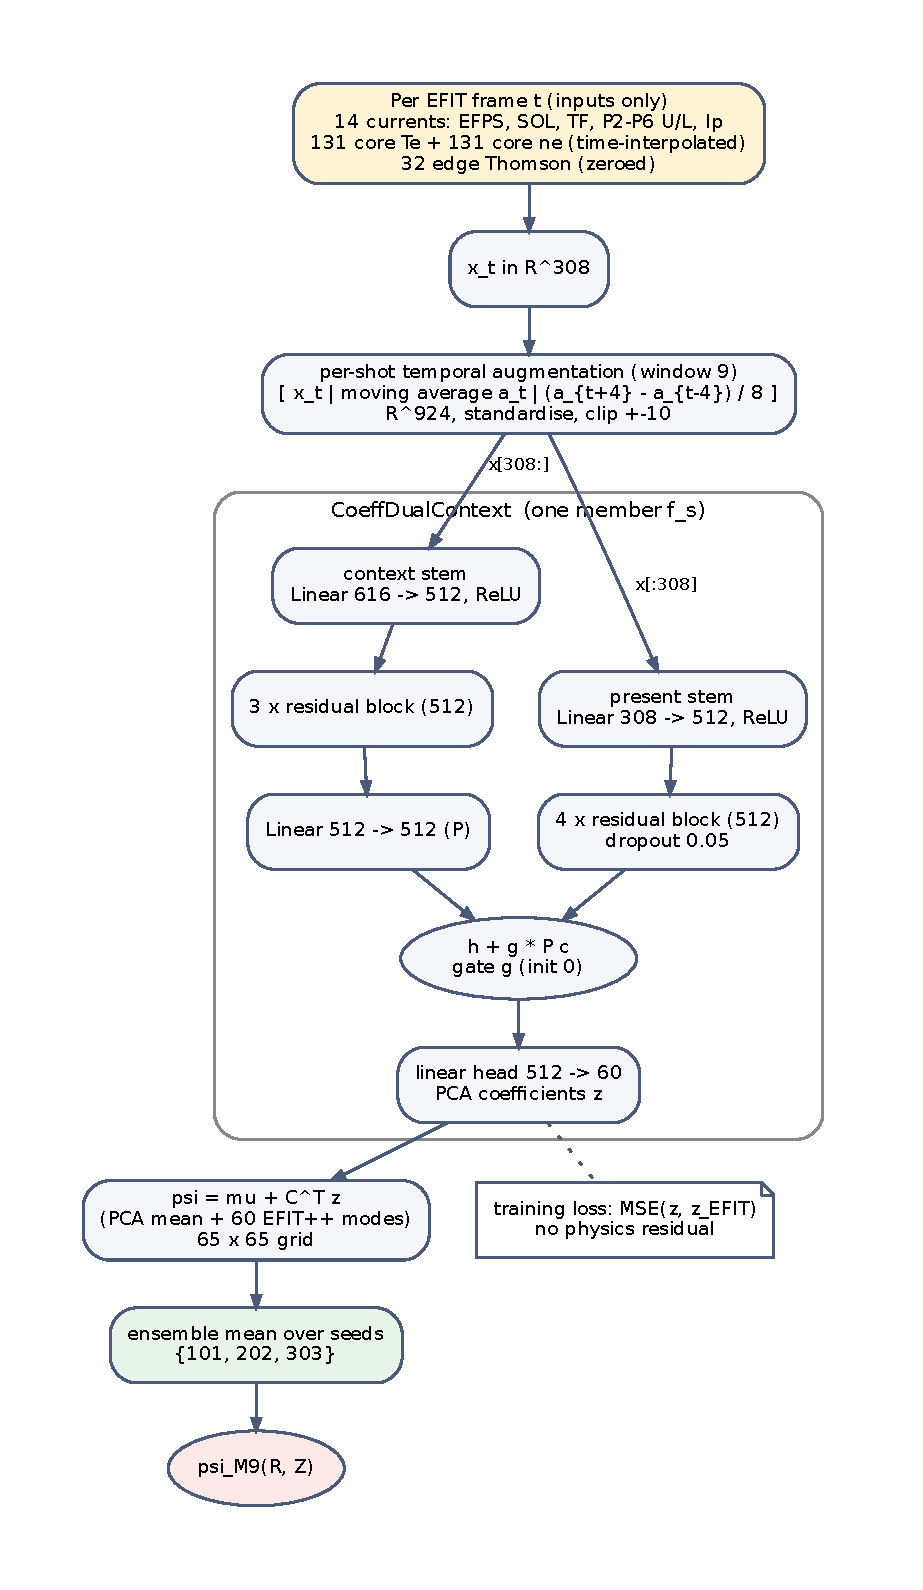
\includegraphics[max width=0.95\linewidth,max height=0.62\textheight,keepaspectratio]{figures/diag_m9_arch.pdf}
\caption{M9 architecture: measured inputs are augmented in time, passed through two residual encoders joined by a zero-initialised gate, mapped linearly to 60 PCA coefficients and reconstructed to the \(65\times65\) grid; three seeds are averaged.}\label{fig:m9}
}
\end{figure}

\hypertarget{what-m9-is-and-is-not}{%
\subsection{What M9 is, and is not}\label{what-m9-is-and-is-not}}

The training script of the source repository is named \nolinkurl{run_crc_feq_pinn_mast.py}, and the model was informally called a ``PCA-PINN''. It is not a physics-informed neural network in the sense of \cite{raissi2019}: the loss is the mean-squared error between predicted and EFIT++ PCA coefficients,

\[
\mathcal L(\theta) = \frac{1}{|B|}\sum_{t\in B}\frac{1}{60}\big\|f_\theta(\tilde x_t) - z_t\big\|_2^{2},
\qquad z_t = C\,(\psi^{\rm EFIT}_t-\mu),
\]

with no Grad--Shafranov residual, boundary condition or conservation term. Any physics in the output is inherited from the EFIT++ training targets and from the PCA subspace they span. We therefore call M9 a \emph{PCA-basis neural surrogate}; the ``pinn'' in the file name is legacy. The network also carries five scalar heads (\(q_{95}\), \(\beta_N\), \(R_{\rm axis}\), \(Z_{\rm axis}\), \(\ell_i\)) that receive no loss and are kept only so that the shipped state dictionaries load.

\hypertarget{pca-basis-of-efit-flux}{%
\subsection{PCA basis of EFIT++ flux}\label{pca-basis-of-efit-flux}}

Each EFIT++ map is flattened to \(\mathbf y_t\in\mathbb R^{4225}\). With \(\mu\) the sample mean and \(C\in\mathbb R^{60\times4225}\) the leading 60 principal directions (orthonormal rows) \cite{pearson1901,hotelling1933}, the reduced representation and its reconstruction are

\begin{equation}
z_t = C(\mathbf y_t-\mu)\in\mathbb R^{60},\qquad \hat{\mathbf y}_t = \mu + C^{\top}z_t .
\label{eq:pca}
\end{equation}

This is the proper orthogonal decomposition of the flux ensemble \cite{berkooz1993}. Because \(C\) has orthonormal rows, MSE on \(z\) equals pixel MSE of the \emph{projected} target. The basis is fitted with randomized SVD \cite{halko2011} (scikit-learn \cite{pedregosa2011}, seed 42, three power iterations) on at most 200,000 frames drawn shot-balanced from the training shots, after the \(|I_p|\) window of the next note. The PCA basis and mean are therefore built from FAIR-MAST EFIT++ labels --- earlier documentation stating that no archive reconstructions were used is incorrect for M9.

\hypertarget{features-and-temporal-context}{%
\subsection{Features and temporal context}\label{features-and-temporal-context}}

For each EFIT frame \(t\) a raw vector \(x_t\in\mathbb R^{308}\) is built:

\begin{longtable}[]{@{}
  >{\raggedright\arraybackslash}p{(\columnwidth - 2\tabcolsep) * \real{0.5000}}
  >{\raggedright\arraybackslash}p{(\columnwidth - 2\tabcolsep) * \real{0.5000}}@{}}
\toprule\noalign{}
\begin{minipage}[b]{\linewidth}\raggedright
slice
\end{minipage} & \begin{minipage}[b]{\linewidth}\raggedright
content
\end{minipage} \\
\midrule\noalign{}
\endhead
\bottomrule\noalign{}
\endlastfoot
0--13 & 13 coil currents (EFPS, SOL, TF, P2--P6 lower/upper) and \(I_p\), linearly interpolated to \(t\) \\
14--275 & 131 core-Thomson \(T_e\) and 131 \(n_e\) channels, interpolated in time (0 outside the Thomson clock) \\
276--307 & 16 + 16 edge-Thomson channels; \textbf{zeroed at inference} (\texttt{mask\_edge}); in training they hold what the ingest carried, which for most archive shots is nothing (60 of the 65 evaluated holdout shots lacked edge Thomson in the ingest) \\
\end{longtable}

No spatial remapping of the Thomson channels is done; channel index stands in for radius. A per-shot temporal augmentation with window 9 appends the centred moving average \(a_t\) (clamped at the shot edges) and its smoothed central difference \((a_{t+4}-a_{t-4})/8\), giving \(A(x)_t=[x_t\,|\,a_t\,|\,\dot a_t]\in\mathbb R^{924}\). Features are standardised with the training mean and standard deviation and clipped to \(\pm10\): \(\tilde x_t=\mathrm{clip}_{\pm10}\big((A(x)_t-m)/\sigma\big)\).

Since the context uses EFIT frames up to four steps ahead, M9 is a smoother over the shot, not a causal real-time estimator.

\hypertarget{network}{%
\subsection{Network}\label{network}}

Each member \(f_s\) (\texttt{CoeffDualContext}) has two residual encoders \cite{he2016}:

\begin{equation}
\begin{aligned}
h &= \mathrm{Res}^{(4)}_{512}\big(\mathrm{ReLU}(W_h\,\tilde x_{[0,308)})\big), &
c &= \mathrm{Res}^{(3)}_{512}\big(\mathrm{ReLU}(W_c\,\tilde x_{[308,924)})\big),\\
h' &= h + g\,P\,c, & z &= W_z\,h' + b_z\in\mathbb R^{60},
\end{aligned}
\label{eq:net}
\end{equation}

where \(\mathrm{Res}^{(n)}_{512}\) is a stack of \(n\) residual blocks of width 512 with dropout 0.05, \(P\) is a \(512\times512\) linear projection and \(g\) is a scalar gate initialised to 0, so training starts from the present-frame encoder alone and learns how much temporal context to admit. The predicted flux is reconstructed with \eqref{eq:pca}.

\hypertarget{training}{%
\subsection{Training}\label{training}}

The recipe (\nolinkurl{models/m9/train.py}, a port of the original with flags \texttt{-\/-seed\ 42\ -\/-epochs\ 50\ -\/-qc\ -\/-shot-balanced\ -\/-mask-edge\ -\/-win}) is:

\begin{enumerate}
\def\labelenumi{\arabic{enumi}.}
\item
  \textbf{Split} as in Section 2.4: 80 sealed shots, pool of 3,655.
\item
  \textbf{QC:} quarantine a shot if \(\max|\psi|\) exceeds the pool median by more than 10 median absolute deviations, or if it is short, non-finite or constant: 3,622 kept.
\item
  \textbf{\(|I_p|\) window:} 2-means on all keep-shot frame values of \(|I_p|\) (seed 42); frames with \(|I_p|\) at or above the midpoint of the two centres, \(I_p^{\rm lo}=328.7293519015368\) kA, are used. 3,265 shots contribute frames. Limited and diverted frames are both included.
\item
  \textbf{PCA} with \(K=60\) (previous notes).
\item
  \textbf{Validation:} 10\% of the windowed shots (seed-42 shuffle).
\item
  \textbf{Optimisation:} AdamW \cite{loshchilov2019} (learning rate \(10^{-3}\), weight decay \(10^{-4}\)), gradient-norm clip 1.0, batches of 2048 frames drawn shot-balanced (uniform shot, then uniform frame), \(\lceil N_{\rm train}/2048\rceil\) steps per epoch, 50 epochs, keeping the epoch with the lowest validation MSE (46, 49 and 46 for the shipped members). PyTorch \cite{paszke2019}.
\end{enumerate}

During extraction the split, QC keep list and \(I_p^{\rm lo}\) were reproduced exactly and a one-epoch smoke test ran, but a full retrain was not carried out; the shipped weights are verified by sha256 instead (Section 8).

\hypertarget{ensemble}{%
\subsection{Ensemble}\label{ensemble}}

Three members differ only in their initialisation seed \(s\in\{101,202,303\}\) (the data split is shared). The prediction is the mean of the reconstructed maps,

\[
\hat\psi_{\rm M9} = \frac13\sum_{s\in\{101,202,303\}}\Big(\mu+C^{\top}f_s(\tilde x)\Big).
\]

Each checkpoint stores its own \(\mu\), \(C\) and feature statistics, so the average is taken in \(\psi\)-space. The ported inference reproduces the original ensemble output with maximum absolute difference 0 on the three demo shots.

\hypertarget{hybrid-mode-build-and-calibration}{%
\clearpage
\section{Hybrid mode, build and calibration}\label{hybrid-mode-build-and-calibration}}

\hypertarget{hybrid-m9-osf}{%
\subsection{Hybrid M9 + OSF}\label{hybrid-m9-osf}}

The shipped submission recipe combines the two models: the flux map comes from M9, the scalars from OSF after two post-hoc factors,

\[
\psi = \hat\psi_{\rm M9},\qquad
q_{95} = \mathrm{clip}\Big(q_{95}^{\rm OSF}\,\frac{c^{*}}{1.20},\,2,\,25\Big),\qquad
\beta_N = \mathrm{clip}\big(\beta_N^{\rm OSF}\,s^{*},\,0.2,\,5\big),
\]

with \(c^{*}=1.062242\) and \(s^{*}=1.078508\). The OSF read-outs are evaluated on the OSF flux, not on the M9 flux. The factors were obtained from aggregate leaderboard scores on the FEC public-test fold (Section 8); a docstring in the source states \(s^{*}=1.000000\), but the code uses 1.078508.

\hypertarget{build-pipeline}{%
\subsection{Build pipeline}\label{build-pipeline}}

The figure below shows the complete build, from public data to scored predictions and the viewer. Green boxes are OSF parameters, the amber box is the holdout split, red boxes are the prediction/evaluation stages.

\begin{figure}[H]
\hypertarget{fig:pipeline}{%
\centering
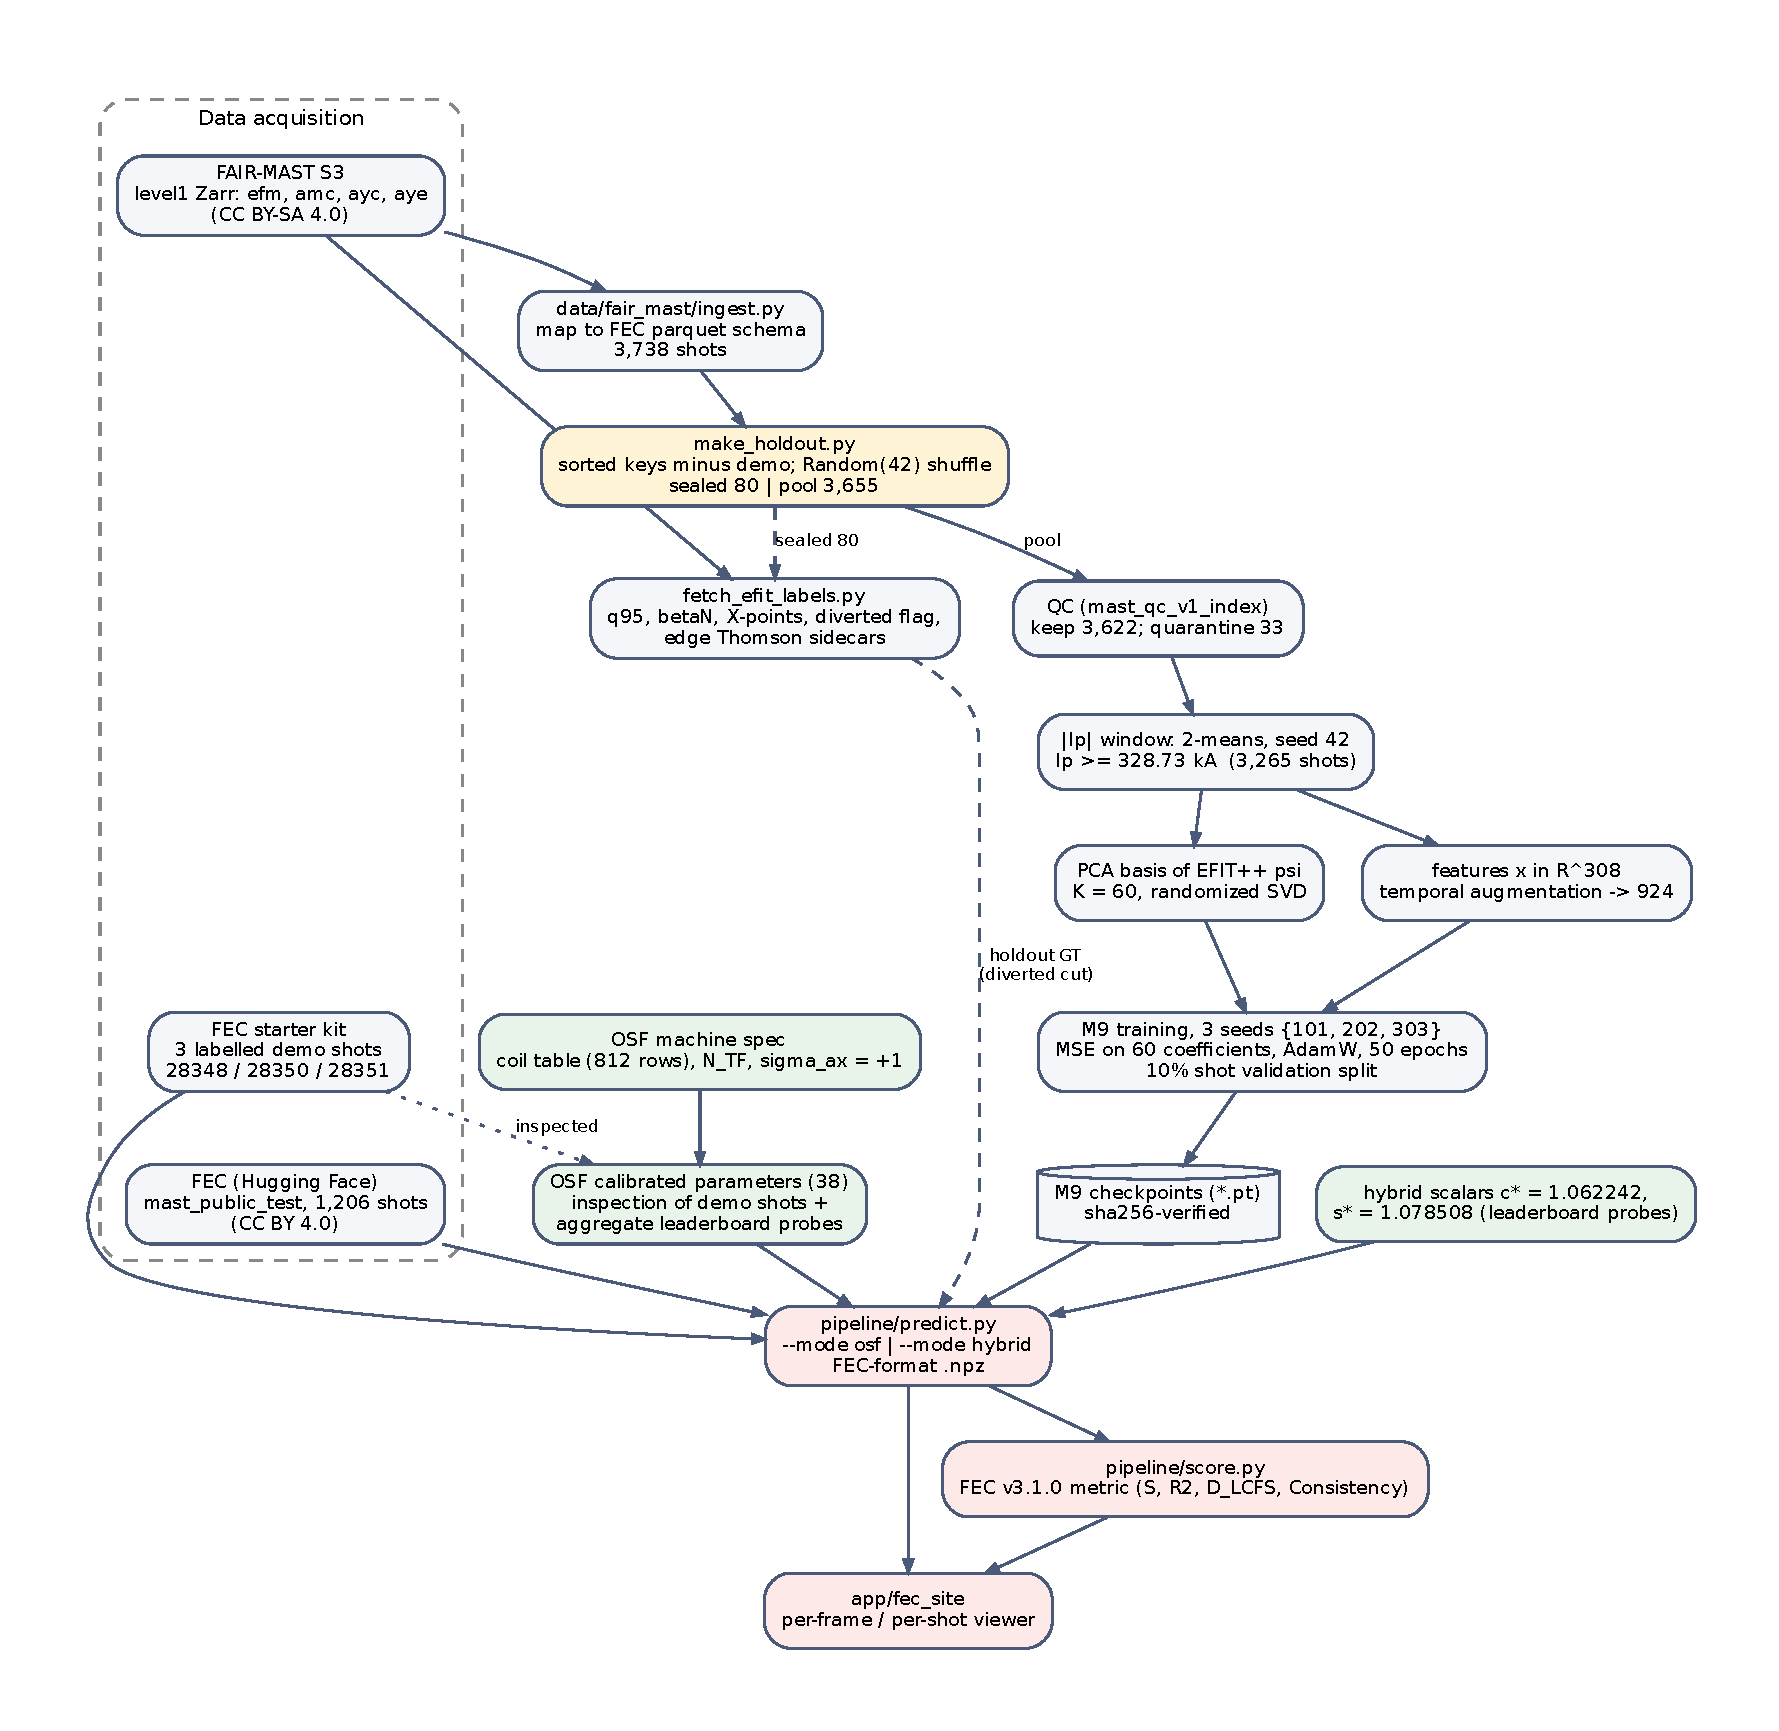
\includegraphics[max width=0.95\linewidth,max height=0.62\textheight,keepaspectratio]{figures/diag_pipeline.pdf}
\caption{Model build and calibration pipeline of the repository. Dashed edges carry labels used only for evaluation; the dotted edge marks the demo shots inspected during OSF calibration.}\label{fig:pipeline}
}
\end{figure}

Labels enter in exactly three places: the M9 PCA basis and loss (archive training pool), the holdout ground truth (sealed shots, evaluation only), and --- informally --- the OSF calibration (next note).

\hypertarget{how-osf-was-calibrated}{%
\subsection{How OSF was calibrated}\label{how-osf-was-calibrated}}

No fitting code exists for OSF; its 38 calibrated values (Section 3.9) are hand-set constants. Per the calibration notes of the source repository they were chosen by

\begin{itemize}
\item
  inspecting physics end-members (ohmic start, solenoid swing, diverted flat-top) on the three labelled starter-kit shots, with \(R^2\) values on those shots quoted to justify shape choices; and
\item
  five aggregate-score probes of the Codabench leaderboard on \texttt{mast\_public\_test}.
\end{itemize}

The demo shots are therefore \emph{not} held out for OSF, and the public-test fold has been used, in aggregate, for tuning. The sealed archive holdout is label-disjoint from all of this, but OSF's global factors were not chosen blind to MAST data. We report the demo-shot scores separately and for reference only.

\hypertarget{commands}{%
\subsection{Commands}\label{commands}}

\begin{verbatim}
python data/fec/fetch.py --demo           # 3 labelled shots
python data/fec/fetch.py --public-test    # 1,206 public-test shots
python data/fair_mast/ingest.py \
    --pool data/fair_mast/mast_pool3.txt --shots 5000
python data/fair_mast/make_holdout.py     # sealed-80 + checks
python data/fair_mast/fetch_efit_labels.py \
    --keys-json data/fair_mast/holdout_seed42.json
python -m models.m9.train --build-cache
python -m models.m9.train --member all
python -m pipeline.predict --split holdout --mode osf
python -m pipeline.predict --split holdout --mode hybrid
python -m pipeline.score outputs/holdout_hybrid.npz
python -m app.fec_site --port 8770
\end{verbatim}

Predictions are FEC-format \nolinkurl{.npz} files with keys \texttt{shot\_XXXX\_psirz} \((T,65,65)\), \texttt{shot\_XXXX\_q95} and \texttt{shot\_XXXX\_betaN} \((T,)\), plus a JSON sidecar giving the shot order. Models only see \texttt{inputs\_only(row)}, which removes every \texttt{efit\_*} label column. Paths may point at an existing data copy through \texttt{FEC\_MAST\_DIR}, \texttt{FEC\_DEMO\_DIR}, \texttt{FAIR\_MAST\_DIR}, \texttt{FAIR\_MAST\_LABELS\_DIR}, \texttt{M9\_WEIGHTS\_DIR} or \texttt{CATSKILLS\_FUSION\_LAB}.

\hypertarget{scoring}{%
\clearpage
\section{Scoring}\label{scoring}}

All results use the FEC scoring code v3.1.0 \cite{fec2026starter}, vendored byte-identical in \nolinkurl{fec_scoring/}; \nolinkurl{pipeline/score.py} ports the fold reduction.

\hypertarget{composite-score}{%
\subsection{Composite score}\label{composite-score}}

For a fold of shots, with \(R^2 = 1-\mathrm{SS}_{\rm res}/\mathrm{SS}_{\rm tot}\) pooled over all frames (and, for \(\psi\), all pixels) of the fold and \(\mathrm{SS}_{\rm tot}\) taken about the ground-truth mean,

\begin{equation}
S = 0.55\,\max(0,R^2_\psi) + 0.15\,\max\Big(0,\tfrac12\big(R^2_{q_{95}}+R^2_{\beta_N}\big)\Big)
+ 0.10\,\big(1-\min(1,D_{\rm LCFS})\big) + 0.20\,\mathrm{Cons}.
\label{eq:score}
\end{equation}

Pooling over the fold means that shots with many frames weigh more, and that \(R^2\) is measured against the variance \emph{across} shots, which is large for \(\psi\) and comparatively small for \(q_{95}\) and \(\beta_N\).

\hypertarget{lcfs-distance}{%
\subsection{LCFS distance}\label{lcfs-distance}}

For each frame the last closed flux surface \(\Gamma\) is extracted from the predicted and from the EFIT++ map by the same code (marching squares inside the vessel envelope). The per-frame distance is the symmetric Hausdorff distance \cite{huttenlocher1993} normalised by the reference geometric major radius of the shot,

\[
d_t = \min\Big(1,\ \frac{d_H(\Gamma^{\rm pred}_t,\Gamma^{\rm EFIT}_t)}{R_{\rm geo}}\Big),\qquad
d_H(A,B)=\max\Big\{\sup_{a\in A}\inf_{b\in B}|a-b|,\ \sup_{b\in B}\inf_{a\in A}|a-b|\Big\}.
\]

\(D_{\rm LCFS}\) averages \(d_t\) over the frames of a shot and then over shots. A failed predicted LCFS counts as \(d_t=1\); frames whose \emph{reference} LCFS cannot be extracted are dropped.

\hypertarget{consistency-scalars}{%
\subsection{Consistency scalars}\label{consistency-scalars}}

Seven scalars are derived from each predicted and each EFIT++ map by the same routine (\nolinkurl{fec_scoring/derive.py}): the magnetic-axis position \(R_{\rm axis}, Z_{\rm axis}\); elongation \(\kappa\) and upper/lower triangularity \(\delta_{\rm top},\delta_{\rm bot}\) from the LCFS extremes; the plasma volume \(V = 2\pi\int_A R\,dR\,dZ\) inside the LCFS; and the internal inductance in the ITER form \(\ell_i(2)=\langle B_p^{2}\rangle_V/(\mu_0I_p/\ell_p)^{2}\), evaluated from \(|\nabla\psi|\). With \(R^2_j\) the pooled \(R^2\) of scalar \(j\),

\[
\mathrm{Cons} = \frac17\sum_{j=1}^{7}\max\big(0,R^2_j\big).
\]

The term measures whether the predicted map is geometrically equivalent to the reconstruction, not whether it is close pixel by pixel.

\hypertarget{sign-and-missing-value-policy}{%
\subsection{Sign and missing-value policy}\label{sign-and-missing-value-policy}}

A single fold-global sign \(s\in\{+1,-1\}\) is chosen to minimise \(\mathrm{SS}_{\rm res}(\psi)\), and the contour work uses the axis sign \(\sigma_{\rm ax}s\); all runs here select \(s=+1\). Non-finite predicted pixels or scalars are replaced by the ground-truth mean, and a derived scalar that cannot be computed from the prediction is replaced in the same way, so failures cost score rather than being skipped.

\hypertarget{results}{%
\clearpage
\section{Results}\label{results}}

Every number in this section is read from the saved prediction and score files (\nolinkurl{outputs/holdout_osf.npz}, \nolinkurl{outputs/holdout_hybrid.score.json} and the corresponding demo files) by \nolinkurl{scripts/make_result_figures.py}, which writes the tables imported below and the figures. The holdout runs were produced on 2026-11-18 with seed 42 and scorer v3.1.0.

\hypertarget{sealed-holdout}{%
\subsection{Sealed holdout}\label{sealed-holdout}}

Sealed-80 holdout (seed 42), restricted to diverted frames: 65 shots, 3,449 frames.

\begin{longtable}[]{@{}
  >{\raggedright\arraybackslash}p{(\columnwidth - 12\tabcolsep) * \real{0.1429}}
  >{\raggedright\arraybackslash}p{(\columnwidth - 12\tabcolsep) * \real{0.1429}}
  >{\raggedright\arraybackslash}p{(\columnwidth - 12\tabcolsep) * \real{0.1429}}
  >{\raggedright\arraybackslash}p{(\columnwidth - 12\tabcolsep) * \real{0.1429}}
  >{\raggedright\arraybackslash}p{(\columnwidth - 12\tabcolsep) * \real{0.1429}}
  >{\raggedright\arraybackslash}p{(\columnwidth - 12\tabcolsep) * \real{0.1429}}
  >{\raggedright\arraybackslash}p{(\columnwidth - 12\tabcolsep) * \real{0.1429}}@{}}
\caption{Composite score and terms on the sealed holdout.}\tabularnewline
\toprule\noalign{}
\begin{minipage}[b]{\linewidth}\raggedright
model
\end{minipage} & \begin{minipage}[b]{\linewidth}\raggedright
\(S\)
\end{minipage} & \begin{minipage}[b]{\linewidth}\raggedright
\(R^2_\psi\)
\end{minipage} & \begin{minipage}[b]{\linewidth}\raggedright
\(R^2_{q_{95}}\)
\end{minipage} & \begin{minipage}[b]{\linewidth}\raggedright
\(R^2_{\beta_N}\)
\end{minipage} & \begin{minipage}[b]{\linewidth}\raggedright
\(1-D_{\rm LCFS}\)
\end{minipage} & \begin{minipage}[b]{\linewidth}\raggedright
Consistency
\end{minipage} \\
\midrule\noalign{}
\endfirsthead
\toprule\noalign{}
\begin{minipage}[b]{\linewidth}\raggedright
model
\end{minipage} & \begin{minipage}[b]{\linewidth}\raggedright
\(S\)
\end{minipage} & \begin{minipage}[b]{\linewidth}\raggedright
\(R^2_\psi\)
\end{minipage} & \begin{minipage}[b]{\linewidth}\raggedright
\(R^2_{q_{95}}\)
\end{minipage} & \begin{minipage}[b]{\linewidth}\raggedright
\(R^2_{\beta_N}\)
\end{minipage} & \begin{minipage}[b]{\linewidth}\raggedright
\(1-D_{\rm LCFS}\)
\end{minipage} & \begin{minipage}[b]{\linewidth}\raggedright
Consistency
\end{minipage} \\
\midrule\noalign{}
\endhead
\bottomrule\noalign{}
\endlastfoot
OSF & 0.618634 & 0.917210 & 0.164457 & 0.379077 & 0.734036 & 0.000000 \\
M9 + OSF & 0.862677 & 0.997771 & 0.342298 & 0.394260 & 0.945207 & 0.820703 \\
\end{longtable}

\begin{longtable}[]{@{}
  >{\raggedright\arraybackslash}p{(\columnwidth - 16\tabcolsep) * \real{0.1111}}
  >{\raggedright\arraybackslash}p{(\columnwidth - 16\tabcolsep) * \real{0.1111}}
  >{\raggedright\arraybackslash}p{(\columnwidth - 16\tabcolsep) * \real{0.1111}}
  >{\raggedright\arraybackslash}p{(\columnwidth - 16\tabcolsep) * \real{0.1111}}
  >{\raggedright\arraybackslash}p{(\columnwidth - 16\tabcolsep) * \real{0.1111}}
  >{\raggedright\arraybackslash}p{(\columnwidth - 16\tabcolsep) * \real{0.1111}}
  >{\raggedright\arraybackslash}p{(\columnwidth - 16\tabcolsep) * \real{0.1111}}
  >{\raggedright\arraybackslash}p{(\columnwidth - 16\tabcolsep) * \real{0.1111}}
  >{\raggedright\arraybackslash}p{(\columnwidth - 16\tabcolsep) * \real{0.1111}}@{}}
\caption{Run facts. LCFS fail is the fraction of frames whose predicted LCFS could not be extracted; derive fail the fraction of non-computable consistency scalars.}\tabularnewline
\toprule\noalign{}
\begin{minipage}[b]{\linewidth}\raggedright
split
\end{minipage} & \begin{minipage}[b]{\linewidth}\raggedright
model
\end{minipage} & \begin{minipage}[b]{\linewidth}\raggedright
shots
\end{minipage} & \begin{minipage}[b]{\linewidth}\raggedright
frames
\end{minipage} & \begin{minipage}[b]{\linewidth}\raggedright
\(\psi\) sign
\end{minipage} & \begin{minipage}[b]{\linewidth}\raggedright
LCFS fail
\end{minipage} & \begin{minipage}[b]{\linewidth}\raggedright
derive fail
\end{minipage} & \begin{minipage}[b]{\linewidth}\raggedright
per-shot mean \(R^2_\psi\)
\end{minipage} & \begin{minipage}[b]{\linewidth}\raggedright
scorer
\end{minipage} \\
\midrule\noalign{}
\endfirsthead
\toprule\noalign{}
\begin{minipage}[b]{\linewidth}\raggedright
split
\end{minipage} & \begin{minipage}[b]{\linewidth}\raggedright
model
\end{minipage} & \begin{minipage}[b]{\linewidth}\raggedright
shots
\end{minipage} & \begin{minipage}[b]{\linewidth}\raggedright
frames
\end{minipage} & \begin{minipage}[b]{\linewidth}\raggedright
\(\psi\) sign
\end{minipage} & \begin{minipage}[b]{\linewidth}\raggedright
LCFS fail
\end{minipage} & \begin{minipage}[b]{\linewidth}\raggedright
derive fail
\end{minipage} & \begin{minipage}[b]{\linewidth}\raggedright
per-shot mean \(R^2_\psi\)
\end{minipage} & \begin{minipage}[b]{\linewidth}\raggedright
scorer
\end{minipage} \\
\midrule\noalign{}
\endhead
\bottomrule\noalign{}
\endlastfoot
holdout & OSF & 65 & 3449 & +1 & 0.0000\% & 0.0207\% & 0.913002 & v3.1.0 \\
holdout & M9 + OSF & 65 & 3449 & +1 & 0.0000\% & 0.0041\% & 0.996645 & v3.1.0 \\
demo & OSF & 3 & 115 & +1 & 0.0000\% & 0.0000\% & 0.981975 & v3.1.0 \\
demo & M9 + OSF & 3 & 115 & +1 & 0.0000\% & 0.0000\% & 0.998571 & v3.1.0 \\
\end{longtable}

M9 + OSF improves every term. The flux itself is nearly solved by M9 (\(R^2_\psi=0.997771\), pooled; per-shot mean 0.996645), and the LCFS distance falls from 0.266 to 0.055 of the major radius. OSF, with no flux labels at all, reaches \(R^2_\psi=0.917210\) but its geometry is biased enough that every consistency \(R^2\) is negative. The scalar term is weak for both, because both use the OSF read-outs.

\hypertarget{consistency-components}{%
\subsection{Consistency components}\label{consistency-components}}

Pooled \(R^2\) of the seven derived scalars on the sealed holdout (before the \(\max(0,\cdot)\) of the Consistency term):

\begin{longtable}[]{@{}
  >{\raggedright\arraybackslash}p{(\columnwidth - 14\tabcolsep) * \real{0.1250}}
  >{\raggedright\arraybackslash}p{(\columnwidth - 14\tabcolsep) * \real{0.1250}}
  >{\raggedright\arraybackslash}p{(\columnwidth - 14\tabcolsep) * \real{0.1250}}
  >{\raggedright\arraybackslash}p{(\columnwidth - 14\tabcolsep) * \real{0.1250}}
  >{\raggedright\arraybackslash}p{(\columnwidth - 14\tabcolsep) * \real{0.1250}}
  >{\raggedright\arraybackslash}p{(\columnwidth - 14\tabcolsep) * \real{0.1250}}
  >{\raggedright\arraybackslash}p{(\columnwidth - 14\tabcolsep) * \real{0.1250}}
  >{\raggedright\arraybackslash}p{(\columnwidth - 14\tabcolsep) * \real{0.1250}}@{}}
\caption{Consistency components on the sealed holdout.}\tabularnewline
\toprule\noalign{}
\begin{minipage}[b]{\linewidth}\raggedright
model
\end{minipage} & \begin{minipage}[b]{\linewidth}\raggedright
\(R_{\rm axis}\)
\end{minipage} & \begin{minipage}[b]{\linewidth}\raggedright
\(Z_{\rm axis}\)
\end{minipage} & \begin{minipage}[b]{\linewidth}\raggedright
\(\kappa\)
\end{minipage} & \begin{minipage}[b]{\linewidth}\raggedright
\(\delta_{\rm top}\)
\end{minipage} & \begin{minipage}[b]{\linewidth}\raggedright
\(\delta_{\rm bot}\)
\end{minipage} & \begin{minipage}[b]{\linewidth}\raggedright
\(V\)
\end{minipage} & \begin{minipage}[b]{\linewidth}\raggedright
\(\ell_i\)
\end{minipage} \\
\midrule\noalign{}
\endfirsthead
\toprule\noalign{}
\begin{minipage}[b]{\linewidth}\raggedright
model
\end{minipage} & \begin{minipage}[b]{\linewidth}\raggedright
\(R_{\rm axis}\)
\end{minipage} & \begin{minipage}[b]{\linewidth}\raggedright
\(Z_{\rm axis}\)
\end{minipage} & \begin{minipage}[b]{\linewidth}\raggedright
\(\kappa\)
\end{minipage} & \begin{minipage}[b]{\linewidth}\raggedright
\(\delta_{\rm top}\)
\end{minipage} & \begin{minipage}[b]{\linewidth}\raggedright
\(\delta_{\rm bot}\)
\end{minipage} & \begin{minipage}[b]{\linewidth}\raggedright
\(V\)
\end{minipage} & \begin{minipage}[b]{\linewidth}\raggedright
\(\ell_i\)
\end{minipage} \\
\midrule\noalign{}
\endhead
\bottomrule\noalign{}
\endlastfoot
OSF & -0.492257 & -0.137536 & -0.069541 & -0.502441 & -0.169103 & -2.645417 & -0.278707 \\
M9 + OSF & 0.889709 & 0.904550 & 0.893904 & 0.906330 & 0.577001 & 0.904904 & 0.668520 \\
\end{longtable}

For M9 + OSF the weakest are \(\delta_{\rm bot}\) (0.577001) and \(\ell_i\) (0.668520): the lower X-point region and the current-profile peaking are the least constrained by the inputs. For OSF the volume \(R^2\) of \(-2.645417\) reflects a systematically small LCFS (next note).

\hypertarget{flux-maps-and-per-shot-spread}{%
\subsection{Flux maps and per-shot spread}\label{flux-maps-and-per-shot-spread}}

The example frame below is from the holdout shot whose M9 + OSF per-shot \(R^2_\psi\) is the median among shots with at least 40 frames (shot 30423, per-shot \(R^2_\psi\) 0.928576 for OSF and 0.999028 for M9 + OSF), at the middle diverted frame.

\begin{figure}[H]
\hypertarget{fig:psi}{%
\centering
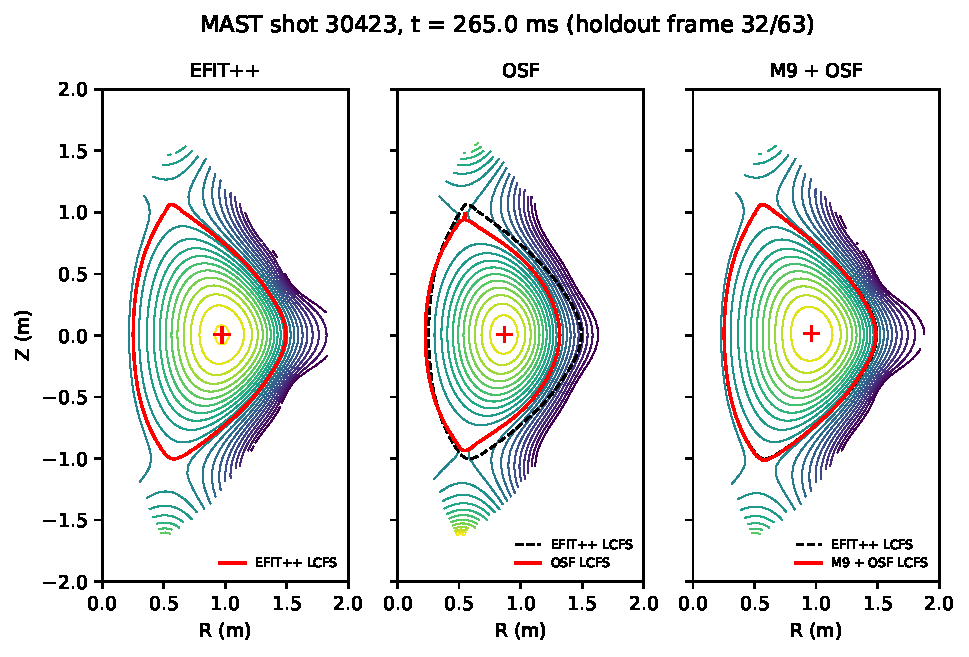
\includegraphics[max width=0.95\linewidth,max height=0.62\textheight,keepaspectratio]{figures/res_psi_compare.pdf}
\caption{EFIT++, OSF and M9 + OSF flux on the vessel mask for MAST shot 30423 at \(t=265\) ms. Red: LCFS of each map; dashed black: EFIT++ LCFS; cross: O-point.}\label{fig:psi}
}
\end{figure}

OSF reproduces the diverted topology, but its LCFS lies inside the EFIT++ LCFS, most visibly on the outboard side and at the top; M9 + OSF overlays EFIT++ almost exactly. The per-shot distributions show the same pattern over the whole holdout:

\begin{figure}[H]
\hypertarget{fig:pershot}{%
\centering
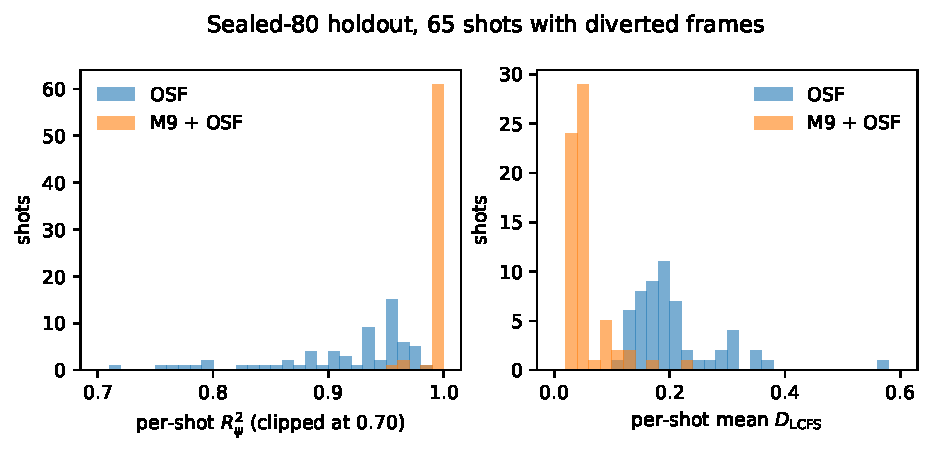
\includegraphics[max width=0.95\linewidth,max height=0.62\textheight,keepaspectratio]{figures/res_pershot_hist.pdf}
\caption{Per-shot \(R^2_\psi\) and per-shot mean \(D_{\rm LCFS}\) on the 65 holdout shots.}\label{fig:pershot}
}
\end{figure}

The eight shots with the lowest M9 + OSF \(R^2_\psi\):

\begin{longtable}[]{@{}
  >{\raggedright\arraybackslash}p{(\columnwidth - 10\tabcolsep) * \real{0.1667}}
  >{\raggedright\arraybackslash}p{(\columnwidth - 10\tabcolsep) * \real{0.1667}}
  >{\raggedright\arraybackslash}p{(\columnwidth - 10\tabcolsep) * \real{0.1667}}
  >{\raggedright\arraybackslash}p{(\columnwidth - 10\tabcolsep) * \real{0.1667}}
  >{\raggedright\arraybackslash}p{(\columnwidth - 10\tabcolsep) * \real{0.1667}}
  >{\raggedright\arraybackslash}p{(\columnwidth - 10\tabcolsep) * \real{0.1667}}@{}}
\caption{Worst holdout shots by M9 + OSF per-shot \(R^2_\psi\).}\tabularnewline
\toprule\noalign{}
\begin{minipage}[b]{\linewidth}\raggedright
shot
\end{minipage} & \begin{minipage}[b]{\linewidth}\raggedright
frames
\end{minipage} & \begin{minipage}[b]{\linewidth}\raggedright
\(R^2_\psi\) OSF
\end{minipage} & \begin{minipage}[b]{\linewidth}\raggedright
\(R^2_\psi\) M9+OSF
\end{minipage} & \begin{minipage}[b]{\linewidth}\raggedright
\(D_{\rm LCFS}\) OSF
\end{minipage} & \begin{minipage}[b]{\linewidth}\raggedright
\(D_{\rm LCFS}\) M9+OSF
\end{minipage} \\
\midrule\noalign{}
\endfirsthead
\toprule\noalign{}
\begin{minipage}[b]{\linewidth}\raggedright
shot
\end{minipage} & \begin{minipage}[b]{\linewidth}\raggedright
frames
\end{minipage} & \begin{minipage}[b]{\linewidth}\raggedright
\(R^2_\psi\) OSF
\end{minipage} & \begin{minipage}[b]{\linewidth}\raggedright
\(R^2_\psi\) M9+OSF
\end{minipage} & \begin{minipage}[b]{\linewidth}\raggedright
\(D_{\rm LCFS}\) OSF
\end{minipage} & \begin{minipage}[b]{\linewidth}\raggedright
\(D_{\rm LCFS}\) M9+OSF
\end{minipage} \\
\midrule\noalign{}
\endhead
\bottomrule\noalign{}
\endlastfoot
27224 & 10 & 0.8403 & 0.9508 & 0.3643 & 0.2353 \\
24463 & 19 & 0.9303 & 0.9632 & 0.2126 & 0.1323 \\
24094 & 75 & 0.9388 & 0.9680 & 0.1829 & 0.0892 \\
23407 & 49 & 0.8797 & 0.9841 & 0.6483 & 0.1047 \\
23882 & 75 & 0.9563 & 0.9916 & 0.1747 & 0.0823 \\
27413 & 56 & 0.8975 & 0.9937 & 0.3433 & 0.1261 \\
23476 & 64 & 0.9596 & 0.9939 & 0.1528 & 0.0463 \\
26464 & 76 & 0.9351 & 0.9946 & 0.1805 & 0.1070 \\
\end{longtable}

\hypertarget{scalars}{%
\subsection{Scalars}\label{scalars}}

\begin{figure}[H]
\hypertarget{fig:scatter}{%
\centering
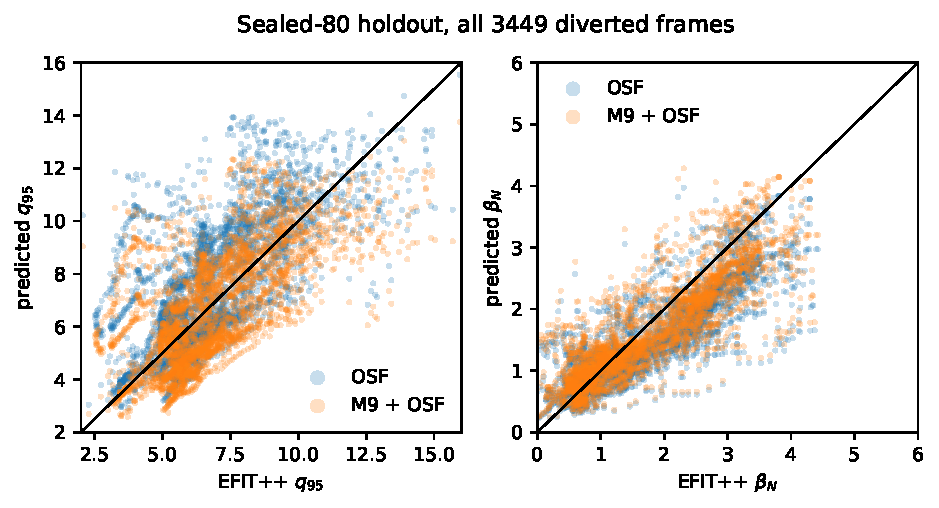
\includegraphics[max width=0.95\linewidth,max height=0.62\textheight,keepaspectratio]{figures/res_scalar_scatter.pdf}
\caption{Predicted versus EFIT++ \(q_{95}\) and \(\beta_N\) over all 3,449 holdout frames.}\label{fig:scatter}
}
\end{figure}

\begin{figure}[H]
\hypertarget{fig:traces}{%
\centering
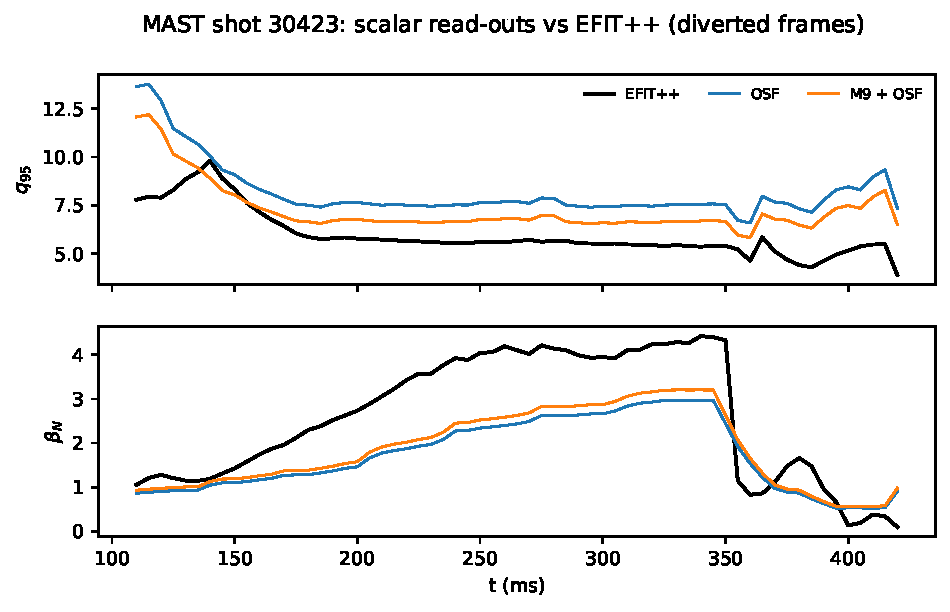
\includegraphics[max width=0.95\linewidth,max height=0.62\textheight,keepaspectratio]{figures/res_scalar_traces.pdf}
\caption{Time traces of \(q_{95}\) and \(\beta_N\) for shot 30423: EFIT++, OSF and M9 + OSF.}\label{fig:traces}
}
\end{figure}

Both read-outs track the trend of EFIT++ within a shot but carry shot-dependent offsets: on shot 30423 the OSF \(q_{95}\) is about 2 too high through the flat-top (M9 + OSF about 1) and \(\beta_N\) is too low at high pressure. Two causes are structural: \(q_{95}\) uses the vacuum \(F\) and an OSF flux whose 95\% surface is too short, and \(\beta_N\) uses a midplane line average of \(2n_eT_e\) rather than a volume average. The hybrid factors \(c^{*}, s^{*}\) only rescale these values, which raises \(R^2_{q_{95}}\) from 0.164457 to 0.342298 and \(R^2_{\beta_N}\) from 0.379077 to 0.394260.

\hypertarget{demo-shots-not-held-out}{%
\subsection{Demo shots (not held out)}\label{demo-shots-not-held-out}}

For reference, the three labelled FEC demo shots (115 frames). These shots informed the OSF calibration and the M9 acceptance gate, so they are \textbf{not} a held-out test.

\begin{longtable}[]{@{}
  >{\raggedright\arraybackslash}p{(\columnwidth - 12\tabcolsep) * \real{0.1429}}
  >{\raggedright\arraybackslash}p{(\columnwidth - 12\tabcolsep) * \real{0.1429}}
  >{\raggedright\arraybackslash}p{(\columnwidth - 12\tabcolsep) * \real{0.1429}}
  >{\raggedright\arraybackslash}p{(\columnwidth - 12\tabcolsep) * \real{0.1429}}
  >{\raggedright\arraybackslash}p{(\columnwidth - 12\tabcolsep) * \real{0.1429}}
  >{\raggedright\arraybackslash}p{(\columnwidth - 12\tabcolsep) * \real{0.1429}}
  >{\raggedright\arraybackslash}p{(\columnwidth - 12\tabcolsep) * \real{0.1429}}@{}}
\caption{Composite score on the three FEC demo shots (not held out).}\tabularnewline
\toprule\noalign{}
\begin{minipage}[b]{\linewidth}\raggedright
model
\end{minipage} & \begin{minipage}[b]{\linewidth}\raggedright
\(S\)
\end{minipage} & \begin{minipage}[b]{\linewidth}\raggedright
\(R^2_\psi\)
\end{minipage} & \begin{minipage}[b]{\linewidth}\raggedright
\(R^2_{q_{95}}\)
\end{minipage} & \begin{minipage}[b]{\linewidth}\raggedright
\(R^2_{\beta_N}\)
\end{minipage} & \begin{minipage}[b]{\linewidth}\raggedright
\(1-D_{\rm LCFS}\)
\end{minipage} & \begin{minipage}[b]{\linewidth}\raggedright
Consistency
\end{minipage} \\
\midrule\noalign{}
\endfirsthead
\toprule\noalign{}
\begin{minipage}[b]{\linewidth}\raggedright
model
\end{minipage} & \begin{minipage}[b]{\linewidth}\raggedright
\(S\)
\end{minipage} & \begin{minipage}[b]{\linewidth}\raggedright
\(R^2_\psi\)
\end{minipage} & \begin{minipage}[b]{\linewidth}\raggedright
\(R^2_{q_{95}}\)
\end{minipage} & \begin{minipage}[b]{\linewidth}\raggedright
\(R^2_{\beta_N}\)
\end{minipage} & \begin{minipage}[b]{\linewidth}\raggedright
\(1-D_{\rm LCFS}\)
\end{minipage} & \begin{minipage}[b]{\linewidth}\raggedright
Consistency
\end{minipage} \\
\midrule\noalign{}
\endhead
\bottomrule\noalign{}
\endlastfoot
OSF & 0.774217 & 0.982004 & 0.841487 & 0.689767 & 0.876086 & 0.158309 \\
M9 + OSF & 0.871921 & 0.998555 & 0.818390 & 0.594122 & 0.955503 & 0.606137 \\
\end{longtable}

\begin{longtable}[]{@{}
  >{\raggedright\arraybackslash}p{(\columnwidth - 14\tabcolsep) * \real{0.1250}}
  >{\raggedright\arraybackslash}p{(\columnwidth - 14\tabcolsep) * \real{0.1250}}
  >{\raggedright\arraybackslash}p{(\columnwidth - 14\tabcolsep) * \real{0.1250}}
  >{\raggedright\arraybackslash}p{(\columnwidth - 14\tabcolsep) * \real{0.1250}}
  >{\raggedright\arraybackslash}p{(\columnwidth - 14\tabcolsep) * \real{0.1250}}
  >{\raggedright\arraybackslash}p{(\columnwidth - 14\tabcolsep) * \real{0.1250}}
  >{\raggedright\arraybackslash}p{(\columnwidth - 14\tabcolsep) * \real{0.1250}}
  >{\raggedright\arraybackslash}p{(\columnwidth - 14\tabcolsep) * \real{0.1250}}@{}}
\caption{Consistency components on the FEC demo shots.}\tabularnewline
\toprule\noalign{}
\begin{minipage}[b]{\linewidth}\raggedright
model
\end{minipage} & \begin{minipage}[b]{\linewidth}\raggedright
\(R_{\rm axis}\)
\end{minipage} & \begin{minipage}[b]{\linewidth}\raggedright
\(Z_{\rm axis}\)
\end{minipage} & \begin{minipage}[b]{\linewidth}\raggedright
\(\kappa\)
\end{minipage} & \begin{minipage}[b]{\linewidth}\raggedright
\(\delta_{\rm top}\)
\end{minipage} & \begin{minipage}[b]{\linewidth}\raggedright
\(\delta_{\rm bot}\)
\end{minipage} & \begin{minipage}[b]{\linewidth}\raggedright
\(V\)
\end{minipage} & \begin{minipage}[b]{\linewidth}\raggedright
\(\ell_i\)
\end{minipage} \\
\midrule\noalign{}
\endfirsthead
\toprule\noalign{}
\begin{minipage}[b]{\linewidth}\raggedright
model
\end{minipage} & \begin{minipage}[b]{\linewidth}\raggedright
\(R_{\rm axis}\)
\end{minipage} & \begin{minipage}[b]{\linewidth}\raggedright
\(Z_{\rm axis}\)
\end{minipage} & \begin{minipage}[b]{\linewidth}\raggedright
\(\kappa\)
\end{minipage} & \begin{minipage}[b]{\linewidth}\raggedright
\(\delta_{\rm top}\)
\end{minipage} & \begin{minipage}[b]{\linewidth}\raggedright
\(\delta_{\rm bot}\)
\end{minipage} & \begin{minipage}[b]{\linewidth}\raggedright
\(V\)
\end{minipage} & \begin{minipage}[b]{\linewidth}\raggedright
\(\ell_i\)
\end{minipage} \\
\midrule\noalign{}
\endhead
\bottomrule\noalign{}
\endlastfoot
OSF & 0.750281 & -0.221832 & -0.594806 & 0.029417 & -0.133666 & -0.024222 & 0.328462 \\
M9 + OSF & 0.891429 & -60.084051 & 0.901171 & 0.596231 & 0.111411 & 0.809666 & 0.933054 \\
\end{longtable}

With only three shots, the pooled \(R^2\) of a scalar with little between-shot variance can be extreme: \(R^2(Z_{\rm axis})=-60.084051\) for M9 + OSF results from a tiny \(\mathrm{SS}_{\rm tot}\), not from a large error. Demo-shot scores overstate holdout performance for the scalars.

\hypertarget{relation-to-the-training-log-figure}{%
\subsection{Relation to the training-log figure}\label{relation-to-the-training-log-figure}}

The M9 training log reports a ``sealed \(R^2\)'' of about 0.378. That figure is a pixel \(R^2\) pooled over \emph{all} 8,161 EFIT slices of the 80 sealed shots --- ramp-up, limited and ramp-down phases included --- and it contains shot 27373, quarantined from training as a QC outlier. Recomputed with the shipped ensemble it is 0.378687, and 0.733818 without shot 27373. On the FEC protocol (diverted slices only) the same ensemble gives the 0.997771 above. The difference is the frame population, not a different model.

\hypertarget{reproducibility-and-limitations}{%
\clearpage
\section{Reproducibility and limitations}\label{reproducibility-and-limitations}}

\hypertarget{verification-of-the-extraction}{%
\subsection{Verification of the extraction}\label{verification-of-the-extraction}}

\begin{longtable}[]{@{}
  >{\raggedright\arraybackslash}p{(\columnwidth - 2\tabcolsep) * \real{0.5000}}
  >{\raggedright\arraybackslash}p{(\columnwidth - 2\tabcolsep) * \real{0.5000}}@{}}
\toprule\noalign{}
\begin{minipage}[b]{\linewidth}\raggedright
check
\end{minipage} & \begin{minipage}[b]{\linewidth}\raggedright
result
\end{minipage} \\
\midrule\noalign{}
\endhead
\bottomrule\noalign{}
\endlastfoot
ported OSF vs original code, 3 demo shots & \(\max|\Delta\psi|\), \(\max|\Delta q_{95}|\), \(\max|\Delta\beta_N|\) = 0 \\
ported M9 inference vs original, 3 demo shots & \(\max|\Delta\psi|\) = 0 \\
\nolinkurl{pipeline.score} vs the source repository's scorer, same predictions & 19 of 19 result fields identical, all four runs \\
M9 split / QC / \(|I_p|\) window recomputed & keep list identical; \(I_p^{\rm lo}=328.7293519015368\) kA \\
shipped M9 checkpoints & sha256 match the source \texttt{SHA256SUMS} \\
FAIR-MAST labels vs FEC demo rows & \(\psi\) bit-identical; \(q_{95}\), \(\beta_N\) and the diverted-frame counts (36/42/37) exact \\
tables of Section 7, regenerated from the saved score files & identical to the repository README \\
\end{longtable}

Not verified: a full M9 retrain to matching weights (only a one-epoch smoke test was run; GPU non-determinism means a retrain reproduces the recipe, not the bytes), and predictions on the public-test fold.

\hypertarget{provenance-documentation-versus-code}{%
\subsection{Provenance: documentation versus code}\label{provenance-documentation-versus-code}}

Reading the source line by line found statements in the earlier documentation that the code does not support. The material ones are:

\begin{enumerate}
\def\labelenumi{\arabic{enumi}.}
\item
  \emph{``No FAIR-MAST EFIT++ / archive reconstructions.''} M9's targets and PCA basis are FAIR-MAST EFIT++ \(\psi\) from 3,622 archive shots; the training code itself notes the pool overlaps the hidden test folds.
\item
  \emph{``\nolinkurl{mast_envelope.npz} not used as a mask.''} OSF's read-outs extract the LCFS with the scorer's envelope mask.
\item
  \emph{``Zero fitting against the 3 demo shots.''} OSF shape choices are justified by demo \(R^2\) values, and the M9 run's acceptance gate is demo \(R^2_\psi\ge0.9976\).
\item
  \emph{``\(c^{*}, s^{*}\) are frozen code hyperparameters.''} They were fitted from leaderboard probes on the public-test fold; one docstring gives \(s^{*}=1.000000\) where the code uses 1.078508.
\item
  \emph{``Paramagnetic \(c=1.20\) baseline''} and \emph{``one-shot''} OSF: neither describes the solver (Sections 3.5 and 3.7).
\item
  \emph{Ingest and demo differ in ``recording / \(\psi\) scale.''} The flux is bit-identical; the frame populations differ.
\item
  \emph{``No magnetic sensors.''} True for model inputs; the EFIT++ labels used them.
\end{enumerate}

The full list of seventeen items is kept in \nolinkurl{DATA_PROVENANCE.md} of the repository.

\hypertarget{limitations}{%
\subsection{Limitations}\label{limitations}}

\begin{itemize}
\item
  \textbf{Labels are magnetics-based.} EFIT++ used probes and flux loops; the task is imputation of a magnetics-constrained reconstruction, and its errors are inherited.
\item
  \textbf{Archive overlap.} Of roughly 4,566 archive shots with EFIT and core Thomson, FEC curated 2,416; the FAIR-MAST training pool very likely contains FEC hidden-fold shots, so M9 is not a zero-shot MAST result in the challenge's sense.
\item
  \textbf{Not fully blind OSF.} OSF's global factors and some shape choices used aggregate public-test scores and the demo shots.
\item
  \textbf{Holdout inputs differ from FEC rows.} The archive ingest resamples the currents differently (up to 44 kA in \(I_p\) on shot 28348, a 0.1 ms clock offset), overlays edge Thomson from \texttt{aye}, and keeps a 131-entry core radius array. Scores on true FEC rows may differ.
\item
  \textbf{Weak scalars.} \(q_{95}\) and \(\beta_N\) come from OSF's simplified read-outs (vacuum \(F\), midplane pressure); M9's scalar heads are untrained.
\item
  \textbf{Non-causal context.} M9 uses EFIT frames up to four steps ahead; it is an offline smoother.
\item
  \textbf{No vessel currents} in OSF, and a fixed elliptical current support.
\item
  \textbf{Retrain not reproduced} end to end; see the previous note.
\end{itemize}

\hypertarget{future-work-an-automated-failure-mode-audit}{%
\clearpage
\section{Future work: an automated failure-mode audit}\label{future-work-an-automated-failure-mode-audit}}

This section is a proposal; none of it has been implemented. During development the author compared imputed and EFIT++ boundaries by eye in the viewer \nolinkurl{app/fec_site}, frame by frame, and inspected the tracked time series for degeneracies. That does not scale to the 3,738 ingested archive shots, let alone all of FAIR-MAST. We propose to make the same inspection systematic.

\hypertarget{what-the-viewer-showed-by-eye}{%
\subsection{What the viewer showed by eye}\label{what-the-viewer-showed-by-eye}}

For one frame of one shot the viewer displays a scorecard (\(S\), \(R^2_\psi\), \(R^2_{q_{95}}\), \(R^2_{\beta_N}\), \(1-D_{\rm LCFS}\), Consistency at fold, shot and frame level); a diagnostics line (frame MSE, a flag for LCFS jumps of 50 mm or more between frames, the Ampère ratio \(\hat I_p/I_p\), validity of equal-\(T_e\) chord pairs on the EFIT and model flux, and the share of the residual lying outside the PCA subspace); side-by-side \(\psi\) panels (EFIT++, model, difference) with LCFS, O-point, X-points and equal-\(T_e\) pairs; residual histograms; \(j_\varphi\) panels; a zoom on the X-point region; and \(q_{95}\), \(\beta_N\) time series against EFIT++ with their difference. Each of these was a judgement made one frame at a time.

\hypertarget{per-frame-audit-quantities}{%
\subsection{Per-frame audit quantities}\label{per-frame-audit-quantities}}

For every frame of every FAIR-MAST shot, compute from the model and EFIT++ maps, with the scorer's own extractors:

\begin{itemize}
\item
  LCFS symmetric Hausdorff distance and the area of the symmetric difference of the two enclosed regions, normalised by the EFIT++ area;
\item
  O-point displacement \(|\Delta(R,Z)_{\rm axis}|\) and X-point displacement for each active X-point;
\item
  topology flags: X-point lost or gained, and limited/diverted flips relative to EFIT++;
\item
  errors of \(\kappa\), \(\delta_{\rm top}\), \(\delta_{\rm bot}\), \(V\) and \(\ell_i\);
\item
  the fraction of the residual outside the 60-mode PCA subspace (what M9 cannot represent);
\item
  for OSF, the Ampère ratio and the number of Picard passes.
\end{itemize}

\hypertarget{time-series-checks}{%
\subsection{Time-series checks}\label{time-series-checks}}

Along each shot, for the boundary and every scalar above, detect

\begin{itemize}
\item
  \textbf{jumps:} frame-to-frame changes exceeding a threshold (e.g.~LCFS moves of 50 mm or more) that EFIT++ does not show;
\item
  \textbf{lag:} the cross-correlation lag between model and EFIT++ series, which exposes the temporal window of M9;
\item
  \textbf{drift:} a slowly growing offset, found by fitting a low-order trend to the difference;
\item
  \textbf{flat-lining or saturation:} stretches where a read-out sits at a clip limit.
\end{itemize}

\hypertarget{failure-classes-and-ranked-reports}{%
\subsection{Failure classes and ranked reports}\label{failure-classes-and-ranked-reports}}

Each frame receives zero or more tags from a small fixed vocabulary --- for example \emph{X-point lost}, \emph{LCFS too wide}, \emph{LCFS too narrow}, \emph{\(\kappa\) biased}, \emph{axis displaced}, \emph{temporal jitter}, \emph{lag}, \emph{drift}, \emph{outside PCA subspace}. Tags are aggregated into ranked worst-shot and worst-frame tables whose rows link directly to the corresponding frame in the viewer, so that inspection by eye is spent on the cases the audit has already identified.

\hypertarget{using-the-audit-in-training}{%
\subsection{Using the audit in training}\label{using-the-audit-in-training}}

The audit turns inspection into training signal:

\begin{enumerate}
\def\labelenumi{\arabic{enumi}.}
\item
  \textbf{Reweighting and targeted sampling} of frames and shots in the over-represented failure classes, in place of uniform shot-balanced sampling;
\item
  \textbf{Shape-aware loss terms} beyond MSE on PCA coefficients --- for example LCFS-distance, X-point and \(\kappa\)/\(\delta\) penalties evaluated through differentiable surrogates, which would also be the first physics-informed element of M9;
\item
  \textbf{A checkpoint gate} defined by failure-class rates on a fixed archive validation set, replacing the current acceptance threshold on the three demo shots (\(R^2_\psi\ge0.9976\)), which is both small and not held out.
\end{enumerate}

\hypertarget{conclusion}{%
\clearpage
\section{Conclusion}\label{conclusion}}

Without magnetic sensors, a forward Grad--Shafranov solver driven by measured coil currents, plasma current and Thomson scattering recovers MAST poloidal flux with \(R^2_\psi=0.917210\) on a sealed archive holdout, but its boundary geometry and scalar read-outs are biased. A PCA-basis neural surrogate trained on EFIT++ flux of 3,622 QC-kept archive shots (3,265 contributing frames after the \(|I_p|\) window) raises \(R^2_\psi\) to 0.997771 and brings the LCFS within about 5\% of the major radius, giving a composite FEC score of 0.862677 in the hybrid configuration. The surrogate learns from magnetics-based reconstructions and is not physics-informed; the remaining weakness is in \(q_{95}\) and \(\beta_N\), which still come from simplified forward read-outs. The repository, the paper sources and all result tables are reproducible from public data, and the documentation now states exactly what each component was fitted to.

\hypertarget{references}{%
\section*{References}\addcontentsline{toc}{section}{References}}

\bibliographystyle{plainnat}
\bibliography{references}

\end{document}
